% !Mode:: "TeX:UTF-8"

\chapter{实证结果}{Empirical Results}
\label{chap04}

本章将报告模型估计的实证结果。本章首先对美国国债券收益率数据做了样本内的拟合处理,随后对模型参数进行估计。

  \begin{align}
   y_{t}(\tau) & = \underset{3\times1} {\mathbf{H}_{t}(\tau)}
   {}'{}  \underset{3\times1} {\mathbf{\beta}_t}
   = \big[\omega(\tau)  \quad
   \frac{1-e^{-\lambda_{t} \tau}} {\lambda_{t} \tau} \quad
   \frac{1-e^{-\lambda_{t} \tau}} {\lambda_{t} \tau} - e^{-\lambda_{t} \tau} \big]
   \begin{bmatrix}
     MY_t \\
     \beta_{2t}\\
     \beta_{3t}
   \end{bmatrix}.
  % \tag{\ref{subsection:The Model:y}$'$} \nonumber \\
 \end{align}

    上文已经说明,\dns 所刻画的收益率曲线的动态特征由模型的参数变量决定。与\citeai{diebold2006forecasting}一致,本文设定\cneqref{subsection:The Model:y}中的两个影响因子服从一个向量自回归过程(VAR),
 \begin{align}\label{var2}
   \mathbf{\beta}_t &=\mathbf{\mu}+\mathbf{\Phi}(L)\mathbf{\beta}_{t-1} + \mathbf{\eps}_t,
 \end{align}
 式中~$\mathbf{\beta}_t = \big[\beta_{2t}, \beta_{3t}\big]'$,$\mathbf{\eps}_t$~服从多元高斯分布,$\mathbf{\eps}_t \sim \mathcal{N}(0,\mathbf{\Omega})$。 未知参数为~$\{\mathbf{\mu}, \mathbf{\Phi}, \mathbf{\Omega}\}$。 其中,模型参数~$\mathbf{\beta}_t$~的~OLS~估计由两步最小二乘法得到:
 
  \begin{align}\label{ols}
   \mathbf{Y} &= \mathbf{G}\mathbf{\beta} ,\quad
   \mathbf{y_t(\tau)}  =
     \begin{pmatrix}
       y_t(1) \\
       y_t(3) \\
       \vdots \\
       y_t(120) \\
     \end{pmatrix},\quad
   \mathbf{G} = 
     \begin{pmatrix}
        \frac{1-e^{-\lambda_{t} }} {\lambda_{t}  } & \frac{1-e^{-\lambda_{t}  }} {\lambda_{t}  } - e^{-\lambda_{t}  } \\
        \frac{1-e^{-3\lambda_{t}  }} {3\lambda_{t} } & \frac{1-e^{-3\lambda_{t}  }} {3\lambda_{t}  } - e^{-3\lambda_{t} } \\
         \vdots &  \vdots\\
        \frac{1-e^{-120\lambda_{t} }} {120\lambda_{t}  } & \frac{1-e^{-120\lambda_{t} }} {120\lambda_{t} } - e^{-120\lambda_{t}} \\
     \end{pmatrix} \\
     \Rightarrow 
     \hat{\mathbf{\beta}}_t &= ( \mathbf{G} '  \mathbf{G})^{-1}  \mathbf{G}'\mathbf{Y}_t .
  \end{align}
 
 这样便构成了两步估计法:(1)先采用最大释然函数估计法,利用实际的收益率曲线对模型参数进行估计,得到~$\hat{\mathbf{\beta}}_t$~;(2)第二步则对参数的向量自回归估计未知参数~$\{\hat{\mathbf{\mu}}, \hat{\mathbf{\Phi}}, \hat{\mathbf{\Omega}}\}$。  设定模型参数服从一个向量自回归过程不仅能够在参数估计上提供便利,这也意味着对收益率曲线的预测等同于对参数动态特征的刻画。这将在下文中具体论述。
 
 \begin{lstlisting}[language=R]
 setwd("/home/william/Desktop/Thesis_XeTex/")

 data <- read.table("data", header = TRUE)
 data <- data[1:372,-1]    

 n.data <- nrow(data)                   ## number of data
 tau <- c(1, 3, 6, 9, 12, 15, 18, 21, 24, 30, 36,
          48, 60, 72, 84, 96, 108, 120)
 n.tau <- length(tau)                  ## number of maturity
 lambda <- 0.0609   ## As in Diebold-Li(2006)
 #######################################
 yld <- as.matrix(data[,1:18])
 my <- as.matrix(data[,22:39])

 M <- matrix(, nrow = 18, ncol = 2) 
 rownames(M) <- c("1m", "3m", "6", "9m", "12m", "15m", "18m", "21m", "24m", "30m", "36m", "48m", "60m", "72m", "84m", "96m", "108m", "120m")
 
 for (i in 1:18){
   M[i,1] = ( 1 - exp(-lambda * tau[i]) ) / ( lambda * tau[i] )
   M[i,2] = ( 1 - exp(-lambda * tau[i]) ) / ( lambda * tau[i] ) - exp( - lambda * tau[i]) 
 }
 
 Beta <- matrix(, nrow = n.data, ncol = 2)
 colnames(Beta) <- c("beta2", "beta3")
 
 for (i in 1:n.data){
   Beta[i,] <- coef( lm(yld[i, 1:18] ~ M -1) )   ## no intercept
 }
 \end{lstlisting}

 模型中代表长期均衡利率水平的缓慢演变过程的成分,$K_t(\tau)$,则可以通过如下估计:
  \begin{align}
    \hat{K}_t & = \hat{\omega}_t  MY_t(\tau).
  \end{align}
  
  \begin{lstlisting}[language=R]
   yld.tilde <- yld - Beta %*% t(M)
   yld.tilde <- ts(yld.tilde,start=c(1970, 1), end=c(2000, 12), frequency=12)
   
   w <-matrix(, nrow = 18, ncol = 1)  ## demographic loadings
   for ( i in 1:18 ){
     w[i] <- coef(lm(yld.tilde[,i] ~ my[,i] - 1))
   }
   
   yld.fit <- matrix(, nrow = n.data, ncol = 18)
   for (j in 1:n.data){
     for (i in 1:18){
       yld.fit[j,i] <- w[i] * my[j,i] + M[i,1] * Beta[j,1] + M[i,2] * Beta[j,2]
     }
   }
  \end{lstlisting}
  
\section{模型参数估计}{Parameters Estimation}

模型需要估计的参数,$\hat{\mathbf{\beta}}_t=(\beta_{2t}, \beta_{3t})'$,由\cneqref{ols}得到。
 \begin{align}
    \hat{\mathbf{\beta}}_t &= ( \mathbf{G}_{t} '  \mathbf{G}_{t})^{-1}  \mathbf{G}_{t}'\mathbf{Y}_t,
 \end{align}
式中~$\mathbf{G}_{t}(\tau)=\big[
   \frac{1-e^{-\lambda_{t} \tau}} {\lambda_{t} \tau},
   \frac{1-e^{-\lambda_{t} \tau}} {\lambda_{t} \tau} - e^{-\lambda_{t} \tau} \big]'$,$\mathbf{Y}_t$~为不同期限的实际国债券的收益率向量。
   
   \subsection{斜率因子与曲度因子}{Slope and Curvature Factors}
   通过两步最小二乘法,我们可以得到斜率因子($\beta_{2t}$)与曲度因子子($\beta_{3t}$)的参数估计值。
%%------------------------------------------------------------------------
  \begin{center}
  \begin{threeparttable}\vspace{-1cm}
  %%
 \caption{模型参数估计结果}
 \label{summarystat2}
 \renewcommand{\arraystretch}{1.2} \arrayrulewidth=0.8pt \tabcolsep=6pt
 \begin{tabular}{c c c c c c c c c c c }
   \hline \hline
 $\hat{\mathbf{\beta}}_t$ & Mean & SD & Min & Max
   & $\hat{\rho}(1)$ & $\hat{\rho}(3)$ & $\hat{\rho}(12)$ & $\hat{\rho}(30)$ \\
   \hline \renewcommand{\arraystretch}{1}
$\hat{\beta}_{2t}$& 2.48 & 2.13 & $-$1.42 & 10.65 & 0.955 & 0.852 & 0.579  & 0.049 \\
$\hat{\beta}_{3t}$& 25.53 & 7.30 & \hspace{.5ex}14.22 & 49.97 & 0.976 & 0.927 & 0.760 & 0.540\\
   \hline \hline
 \end{tabular}
\end{threeparttable}
\end{center}
%%------------------------------------------------------------------------
\tabref{summarystat2}给出了相关的统计结果。可以看到,两个因子在短期内的自相关系数较高,到$12$期后仍然分别为$(0.579,0.760) $。\figref{Rplot11}与\figref{Rplot12}画出了相应的自相关及偏相关系数。
 %------------------------------------------------------
       \begin{figure}%[!h]
    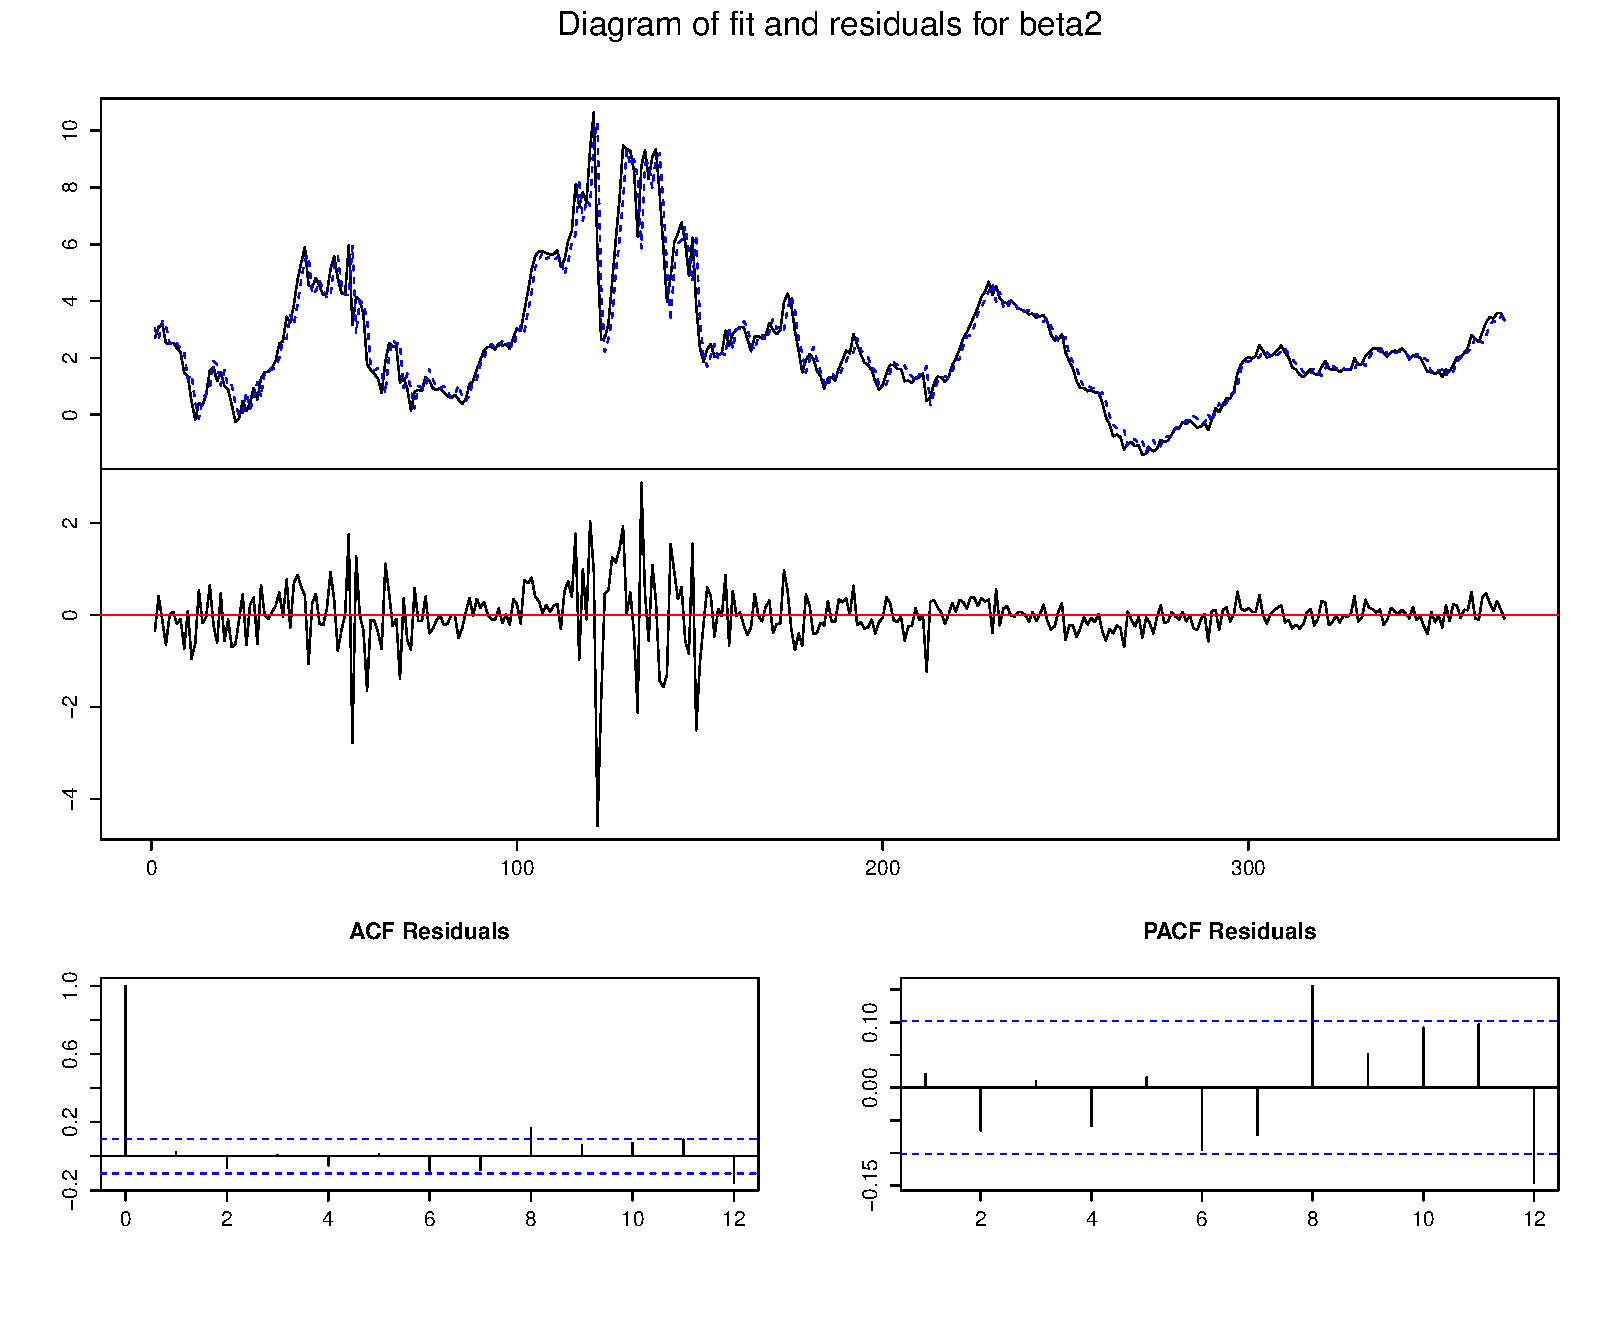
\includegraphics[width=15cm,height=15cm]{figures/Rplot11}
   \caption{斜率因子$\hat{\beta}_{2t}$}
   \label{Rplot11}
  \end{figure}
 %------------------------------------------------------
 %------------------------------------------------------
       \begin{figure}%[!h]
    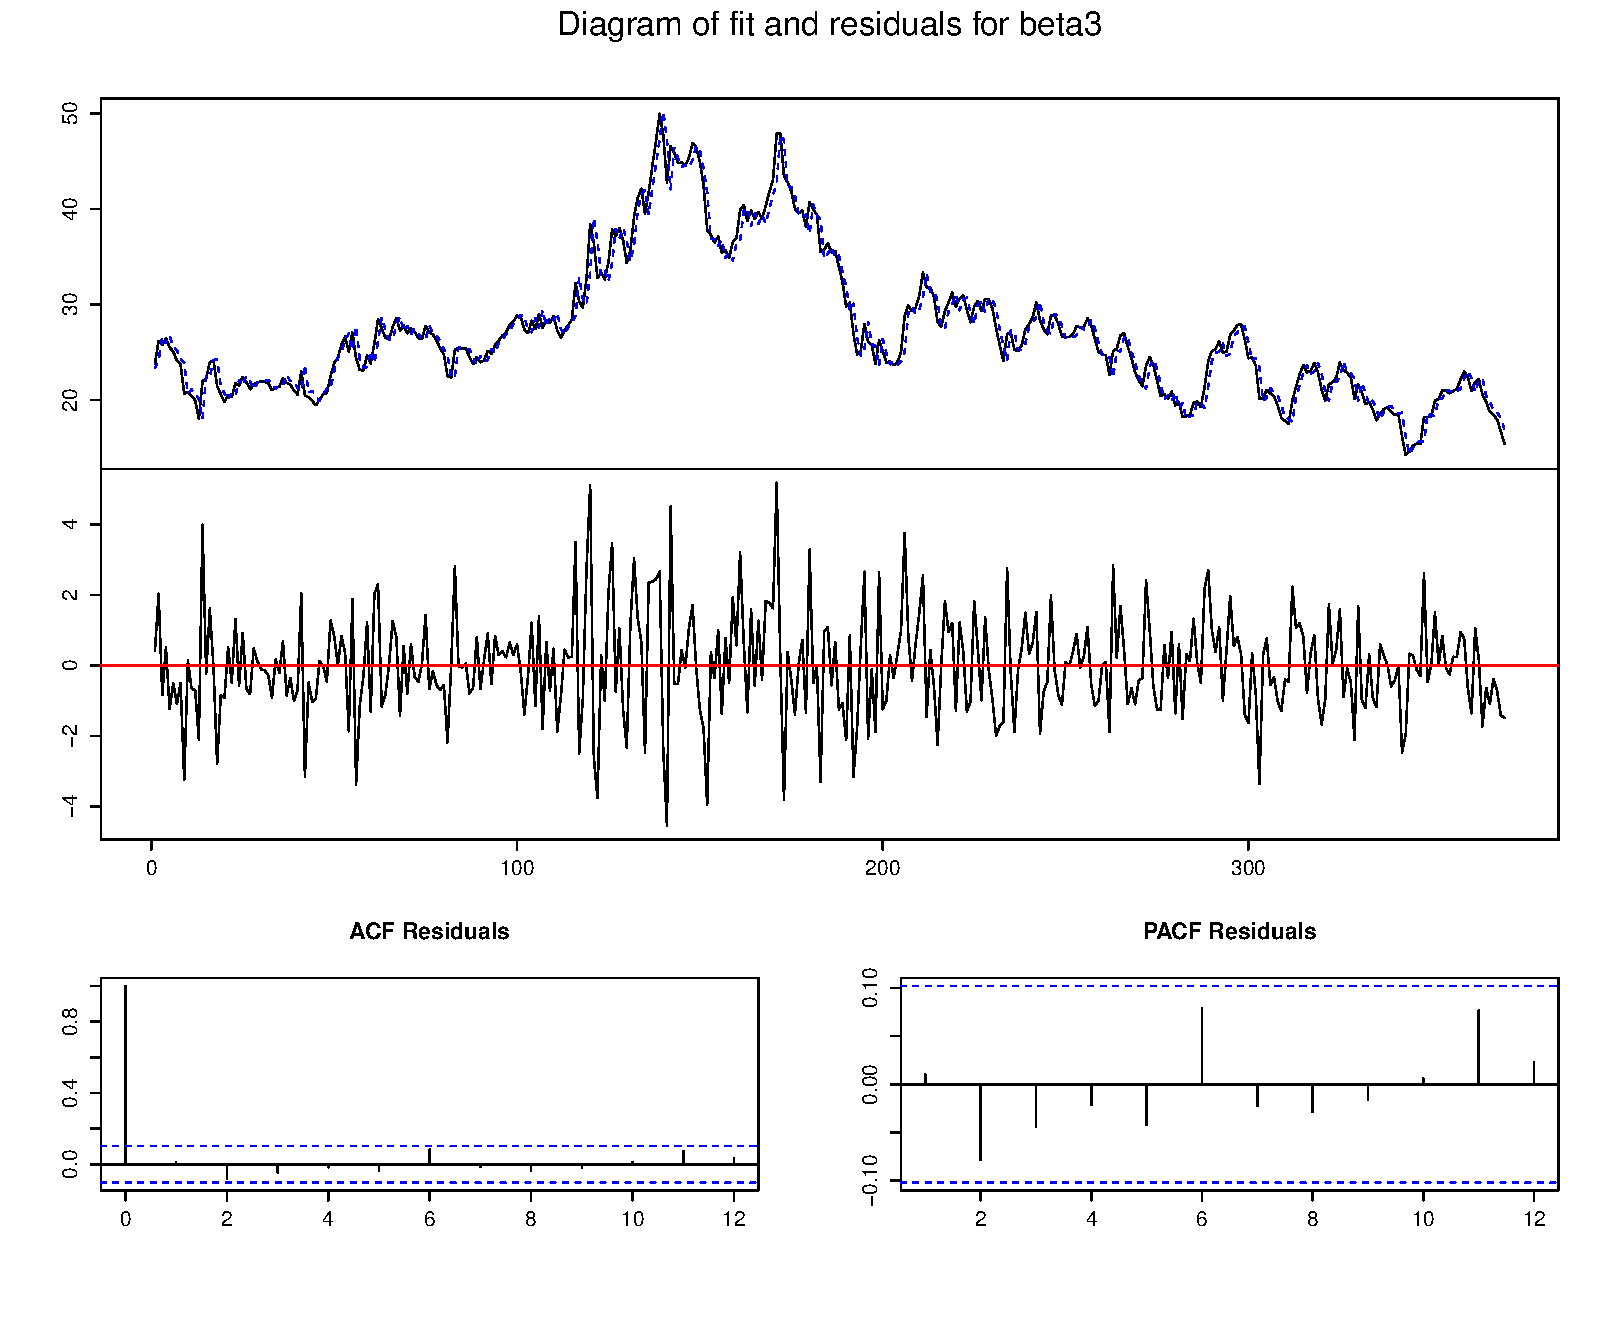
\includegraphics[width=15cm,height=15cm]{figures/Rplot12}
   \caption{曲度因子$\hat{\beta}_{3t}$}
   \label{Rplot12}
  \end{figure}
 %------------------------------------------------------
 
 传统的计量回归方法通常要求所使用的时间序列必须是一个平稳的随机过程。然而,现实中许多的经济现象往往都不平稳的过程,产生了许多的不平稳时序数据,甚至是整个经济系统偶尔伴随有结构性突变。比如,我们在上面的分析中应当注意到,影响整个收益率曲线的因素可以分为两大类:一个是具有平稳性质的、在一个世代叠交的频率上发生的人口因素;另外的这是影响利率中短期动态特征的、非平稳的斜率因子与曲度因子。对于后者,倘若采取传统的普通最小二乘法,就会出现「伪」回归和「无意义」回归的现象。有鉴于此,\citeai{engle1987co}首先提出了一种处理非平稳序列的全新的研究方法——协整(co-integration)研究方法。为了在下一步对斜度因子与曲度因子做时间序列建模,我们首先需要先其二者进行单位根检验,即检验序列本身是非平稳的,但其一阶差分是平稳的。
 %------------------------------------------------------
 \subsubsection{单位根检验}
 本文采用的是扩展的Dickey-Fuller单位根检验,通常是在时间序列分析当中用来辨识个别变量的样本资料是否存在单根。对于任何一个时间序列,$\{z\}_t^T$,为了验证在其是否存在单位根,可以使用以下回归来检验:
 \begin{align*}
  z_t &= \mu +  c t + \alpha_t z_{t-1} + \sum_{i=1}^{p-1}\phi \Delta z_{t-i} + \epsilon_t \\
  \mbox{H}_o &: \alpha = 1 \quad \mbox{v.s.} \quad \mbox{H}_1 : \alpha < 1 \\
 \end{align*}
 其中,$\Delta z_{j}=z_{j}-z_{j-1}$是$z_t$的差分序列。接受原假设意味着时间序列含有单位根。从\tabref{adf}的检验结果可以得知,两个因子在$5\%$的显著水平上存在单位根的原假设无法拒绝,而一阶差分后可以拒绝非稳态的原假设。因而所有变量序列都是$I(1)$,即均具有单位根。
 %------------------------------------------------------
 \begin{table*}\centering
 \caption{ADF单位根检验}
 \label{adf}
 \renewcommand{\arraystretch}{1.2} 
 \begin{tabular}{@{}c c c c c c @{}}\hline\hline
 \multirow{2}*{$\hat{\mathbf{\beta}}_t$} 
 & \multirow{2}*{Lags} 
 & \multirow{2}*{Test Value} & \multicolumn{3}{c}{Critical Value}\\ \cmidrule{4-6}
      &      &        & $1\%$ & $5\%$ & $10\%$ \\
 \hline \renewcommand{\arraystretch}{1.2} 
 $\hat{\beta}_{2t}$ & $2$ & \hspace{-.5em}$-3.0401$ & $-3.98$ & $-3.42$ & $-3.13$\\
 $\Delta\hat{\beta}_{2t}$ & $1$ & $-14.0956^{***}$ & $-3.44$ & $-2.87$ & $-2.57$\\
 $\hat{\beta}_{3t}$ & $2$ & \hspace{-.5em}$-1.9081$ & $-3.98$ & $-3.42$ & $-3.13$\\
  $\Delta\hat{\beta}_{3t}$ & $1$ & $-14.1453^{***}$ & $-3.44$ & $-2.87$ & $-2.57$\\
 \hline\hline
 \end{tabular}
 \end{table*}
 
  %------------------------------------------------------
  \subsubsection{协整检验}
  由以上的单位根检验我们知道,影响收益率曲线短期动态特征的两个斜率因子与曲度因子的时间序列是一个$I(1)$过程。即它们具备构造协整方程组的必要条件。如果两个(或两个以上)的时间序列是非平稳的,但它们的某种线性组合却是平稳的,则这两个(或两个以上)的非平稳的时间序列之间存在长期的均衡关系(或协整关系)。从经济研究的角度看,两个时间序列之间存在的协整关系意味着我们可以使用一个变量来影响另外的变量,二者之间存在一种相互联系的均衡关系。为此,我们对上述各个变量序列之间做长期的协整分析。
  
   %------------------------------------------------------
  \tabref{cointegration}列出了对\cneqref{var2}做~Johansen~协整检验的结果。结果显示,零阶协整的原假设无法被接受,而一阶协整的原假设无法被拒绝。
 %------------------------------------------------------
   \begin{table*}\centering
   \caption{Johansen~协整检验}
   \label{cointegration}
   \renewcommand{\arraystretch}{1.2} 
   \begin{tabular}{@{}c c c c c c@{}}\hline\hline
   \multirow{2}*{$\mathcal{H}_0$} 
   & \multicolumn{2}{c}{Test Value} 
   &  \multicolumn{3}{c}{Critical Value}\\ \cmidrule{2-3} \cmidrule{4-6}
        &   $p=2$   &   $p=3$     & $90\%$ & $95\%$ & $99\%$ \\
   \hline \renewcommand{\arraystretch}{1.2} 
   $r=1$ & \hspace{.5em}$6.52$ & $\hspace{.5em}5.32$ & $10.49$ & $12.25$ & $16.26$\\
   $r=0$ & $17.26$ & $14.43$ & $16.85$ & $18.96$ & $23.65$\\
   \hline\hline
   \end{tabular}
   \end{table*}
  
  %------------------------------------------------------
  \subsubsection{选择滞后期} 
  我们已经知道收益率曲线中的两个斜率因子与曲度因子为一个$I(1)$的协整关系。为了建立一个向量自回归模型($VAR(p)$),我们还需要恰当的选择其滞后项,即利用适当的信息原则确定~VAR~的阶数。这包括AIC、BIC、HQ等多种信息准则。由于各个信息准则所关注的侧重点不同,并没有一个固定的模式。一方面,主要考虑到模型不能过于复杂,如果选择的滞后期过多,则模型估计比较困难;另一方面,我们也同时兼顾其他信息准则。根据\tabref{varlag}的检验结果,HQ和SC准则都给出的最优滞后期是1期,而AIC和FPE为8期,考虑到后者建模过于复杂。由于各个信息准则所关注的侧重点不同,并没有一个固定的模式。因此,这里选择向量自回归滞后期为1期,即$\Delta \beta_t \sim VAR(1)$。
  % Table created by stargazer v.5.0 by Marek Hlavac, Harvard University. E-mail: hlavac at fas.harvard.edu
  % Date and time: 六,  3月 29, 2014 - 05时08分01秒
     \begin{center}
    \begin{threeparttable}[!htbp] \centering 
    \caption{VAR~滞后阶数} 
    \label{varlag} \tabcolsep=5pt
  \begin{tabular}{@{}lcccccccc@{}} 
    \hline \hline 
  Criteria     & 1 & 2 & 3 & 4 & 5 & 6 & 7 & 8 \\ 
       \hline
AIC(n) & $$-$0.147$$^*$ & $$-$0.150$ & $$-$0.138$ & $$-$0.123$ & $$-$0.133$ & $$-$0.151$ & $$-$0.163$ & $$-$0.167$ \\ 
HQ(n)  & $$-$0.113$$^*$ & $$-$0.099$ & $$-$0.070$ & $$-$0.038$ & $$-$0.031$ & $$-$0.032$ & $$-$0.026$ & $$-$0.013$ \\ 
SC(n)  &  $$-$0.061$$^*$ & $$-$0.022$ & $0.034$ & $0.092$ & $0.125$ & $0.149$ & $0.181$ & $0.220$ \\ 
FPE(n) &  $0.864$ & $0.860$ & $0.871$ & $0.884$ & $0.876$ & $0.860$ & $0.850$ & $0.847$$^*$ \\ 
  \hline\hline  
  \end{tabular}
    \small{%
    \emph{注}: $^*$ $5\%$显著水平上最佳滞后期:
     \begin{tablenotes}
  \item [1]  AIC: Akaike information criterion
  \item [2]  HQ: Hannan-Quinn information criterion	
  \item [3]  SC: Schwarz information criterion  		
  \item [4]  FPE: Final prediction error							
  \end{tablenotes}
  }% 
  \end{threeparttable}
  \end{center}
  
 %------------------------------------------------------
对于任何一个时间序列,$\{\hat{\beta}_{2t},\hat{\beta}_{3t}\}'$,首先对~$\hat{\beta}_{2t}$~和~ $\hat{\beta}_{3t}$~取一阶差分以得到平稳序列:
  \begin{align}\label{var3}
    \begin{bmatrix}
      \Delta \hat{\beta}_{2t} \\
      \Delta \hat{\beta}_{3t} \\
    \end{bmatrix}
    & =
    \mathbf{\mu} + 
    \begin{bmatrix}
     \phi_{11} & \phi_{12} \\
     \phi_{21} & \phi_{22} \\
    \end{bmatrix}
       \begin{bmatrix}
      \Delta  \hat{\beta}_{2,t-1} \\
      \Delta \hat{\beta}_{3,t-1}\\
    \end{bmatrix}+ \mathbf{\eps}_t, \quad \mathbf{\eps}_t\sim \mathcal{N}(0,\Omega).
  \end{align}
令 $\Delta\mathbf{\hat{\beta}}_t=(\Delta\hat{\beta}_{2t},\Delta\hat{\beta}_{3t})'$。
%%---------------------------------------------------------------------------- 
   因此,可以将\cneqref{var3}写做更加紧密的形式:
    \begin{align}\label{var5}
  \Delta\mathbf{\hat{B}}_t &=
    \begin{bmatrix}
      \Delta\mathbf{\hat{\beta}}_t \\ \Delta\mathbf{\hat{\beta}}_{t-1}
    \end{bmatrix}
    = \begin{bmatrix}
      \mathbf{\mu} \\ \mathbf{\underline{0}}
    \end{bmatrix}
    + \begin{bmatrix}
      \mathbf{\hat{\Phi}}_1 & \mathbf{\underline{I}} \\ \mathbf{\underline{I}} & \mathbf{\underline{0}}
    \end{bmatrix}
    \begin{bmatrix}
      \mathbf{\hat{\beta}}_{t-1} \\ \mathbf{\hat{\beta}}_{t-2}
    \end{bmatrix}
    + \begin{bmatrix}
      \mathbf{\eps}_t \\ \mathbf{\underline{0}}
    \end{bmatrix}
    = \mathbf{\tilde{\mu}}  +\mathbf{\hat{\Gamma}} \mathbf{\hat{B}}_{t-1} + \mathbf{\tilde{\eps}}_t,
  \end{align}
  式中,$\mathbf{\hat{B}}_t=[\mathbf{\hat{\beta}}_t, \mathbf{\hat{\beta}}_{t-1}]'$,
  $\mathbf{\tilde{\mu}}=[\mathbf{\hat{\mu}},\mathbf{\underline{0}}]'$,$\mathbf{\hat{\Gamma}}=\begin{bmatrix}
      \mathbf{\hat{\Phi}} & \mathbf{\underline{I}}\\ \mathbf{\underline{I}} & \mathbf{\underline{0}}
    \end{bmatrix}$,
    以及~$ \mathbf{\tilde{\eps}}_t=[\mathbf{\eps}_t,\mathbf{\underline{0}}]'$,即
    \begin{align}
     \Delta\mathbf{\hat{B}}_t &=\mathbf{\tilde{\mu}}  +\mathbf{\hat{\Gamma}} \Delta\mathbf{\hat{B}}_{t-1} + \mathbf{\tilde{\eps}}_t. \tag{\ref{var5}$'$}
    \end{align}
    从而~$h$~期后的预测为
    \begin{align}
   \Delta\mathbf{\hat{B}}_{t+h|t}
    &=\sum_{j=0}^{h-1}\mathbf{\hat{\Gamma}}^j \mathbf{\tilde{\mu}}
     +\mathbf{\hat{\Gamma}}^h \Delta\mathbf{\hat{B}}_t.
   \end{align}
 %------------------------------------------------------
   \begin{center}
  \begin{threeparttable}
 \caption{VAR~参数估计}
 \label{summary_stat2}
 \renewcommand{\arraystretch}{1.2} \arrayrulewidth=0.8pt \tabcolsep=6pt
 \begin{tabular}{@{}c c c c  c c @{}}
   \hline \hline
  & \multicolumn{2}{c}{$\mathbf{\hat{\Phi}}$}
 & $\mathbf{\hat{\mu}}$ & \multicolumn{2}{c}{$\mathbf{\hat{\Omega}}$} \\
   \hline \renewcommand{\arraystretch}{1}
$\Delta\hat{\beta}_{2t}$ & $\underset{(0.0512)}{0.1215}$& $\underset{(0.0220)}{0.0633}$ & $\underset{(0.0323)}{-0.0016}$  & \hspace{0.5ex}$0.3848$&\\
$\Delta\hat{\beta}_{3t}$ & \hspace{-1ex}$\underset{(0.1209)}{-0.0563}$& $\underset{(0.05120)}{0.0937}$ & $\underset{(0.0762)}{-0.0188}$  & \hspace{0.5ex}$0.045$ & 2.147\\
   \hline \hline
 \end{tabular}
  \small{%
  \emph{注}:VAR~的动态过程由\cneqref{var3}表示。括号里报告了标准差。
}%
\end{threeparttable}
\end{center}

经过VAR拟合后,我们得到\figref{Rplot13}和\figref{Rplot14},表明一阶差分后的向量自回归模型是平稳的。
 %------------------------------------------------------
       \begin{figure}%[!h]
    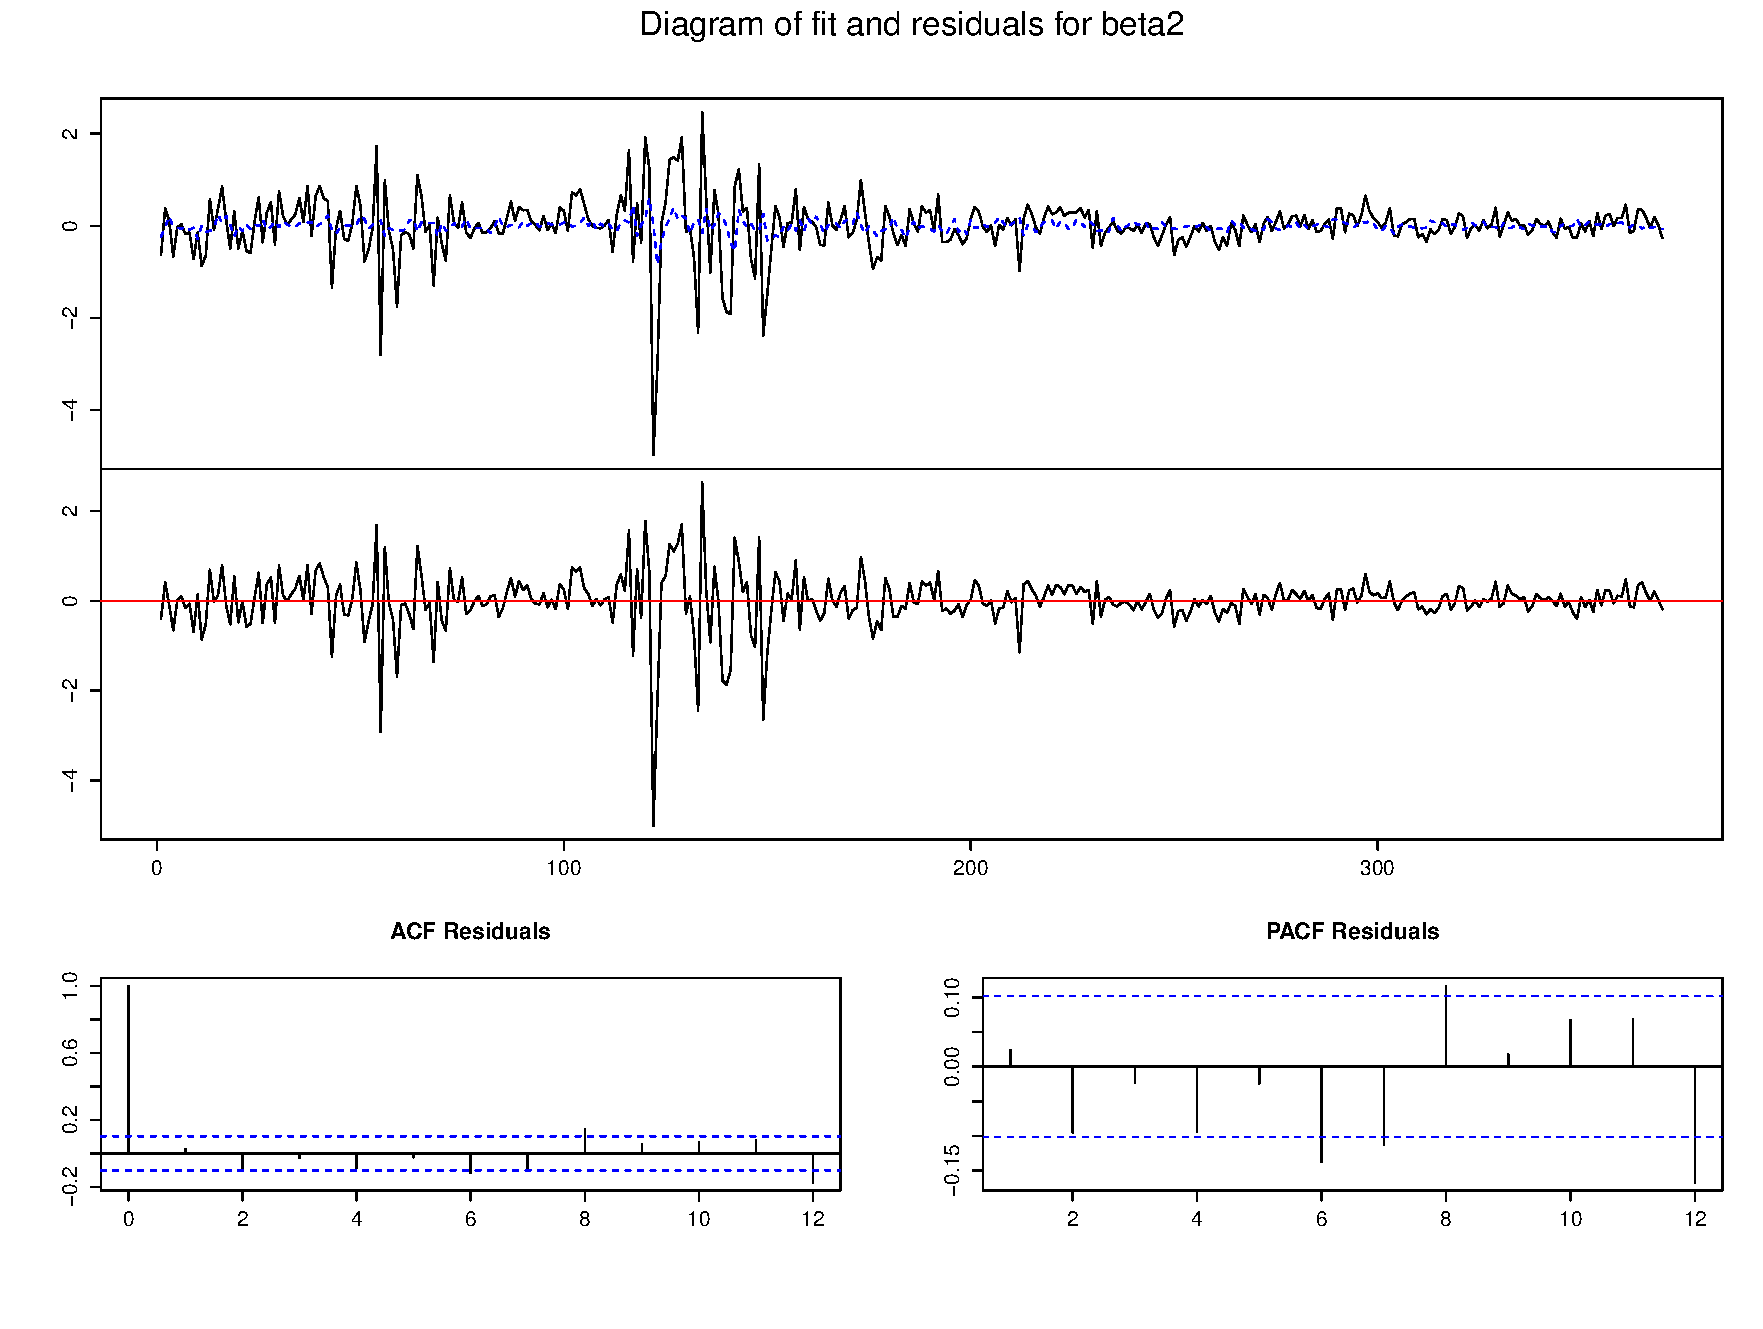
\includegraphics[width=15cm,height=15cm]{figures/Rplot13}
   \caption{一阶差分的斜率因子,$\Delta\hat{\beta}_{2t}$}
   \label{Rplot13}
  \end{figure}
 %------------------------------------------------------
 %------------------------------------------------------
       \begin{figure}%[!h]
    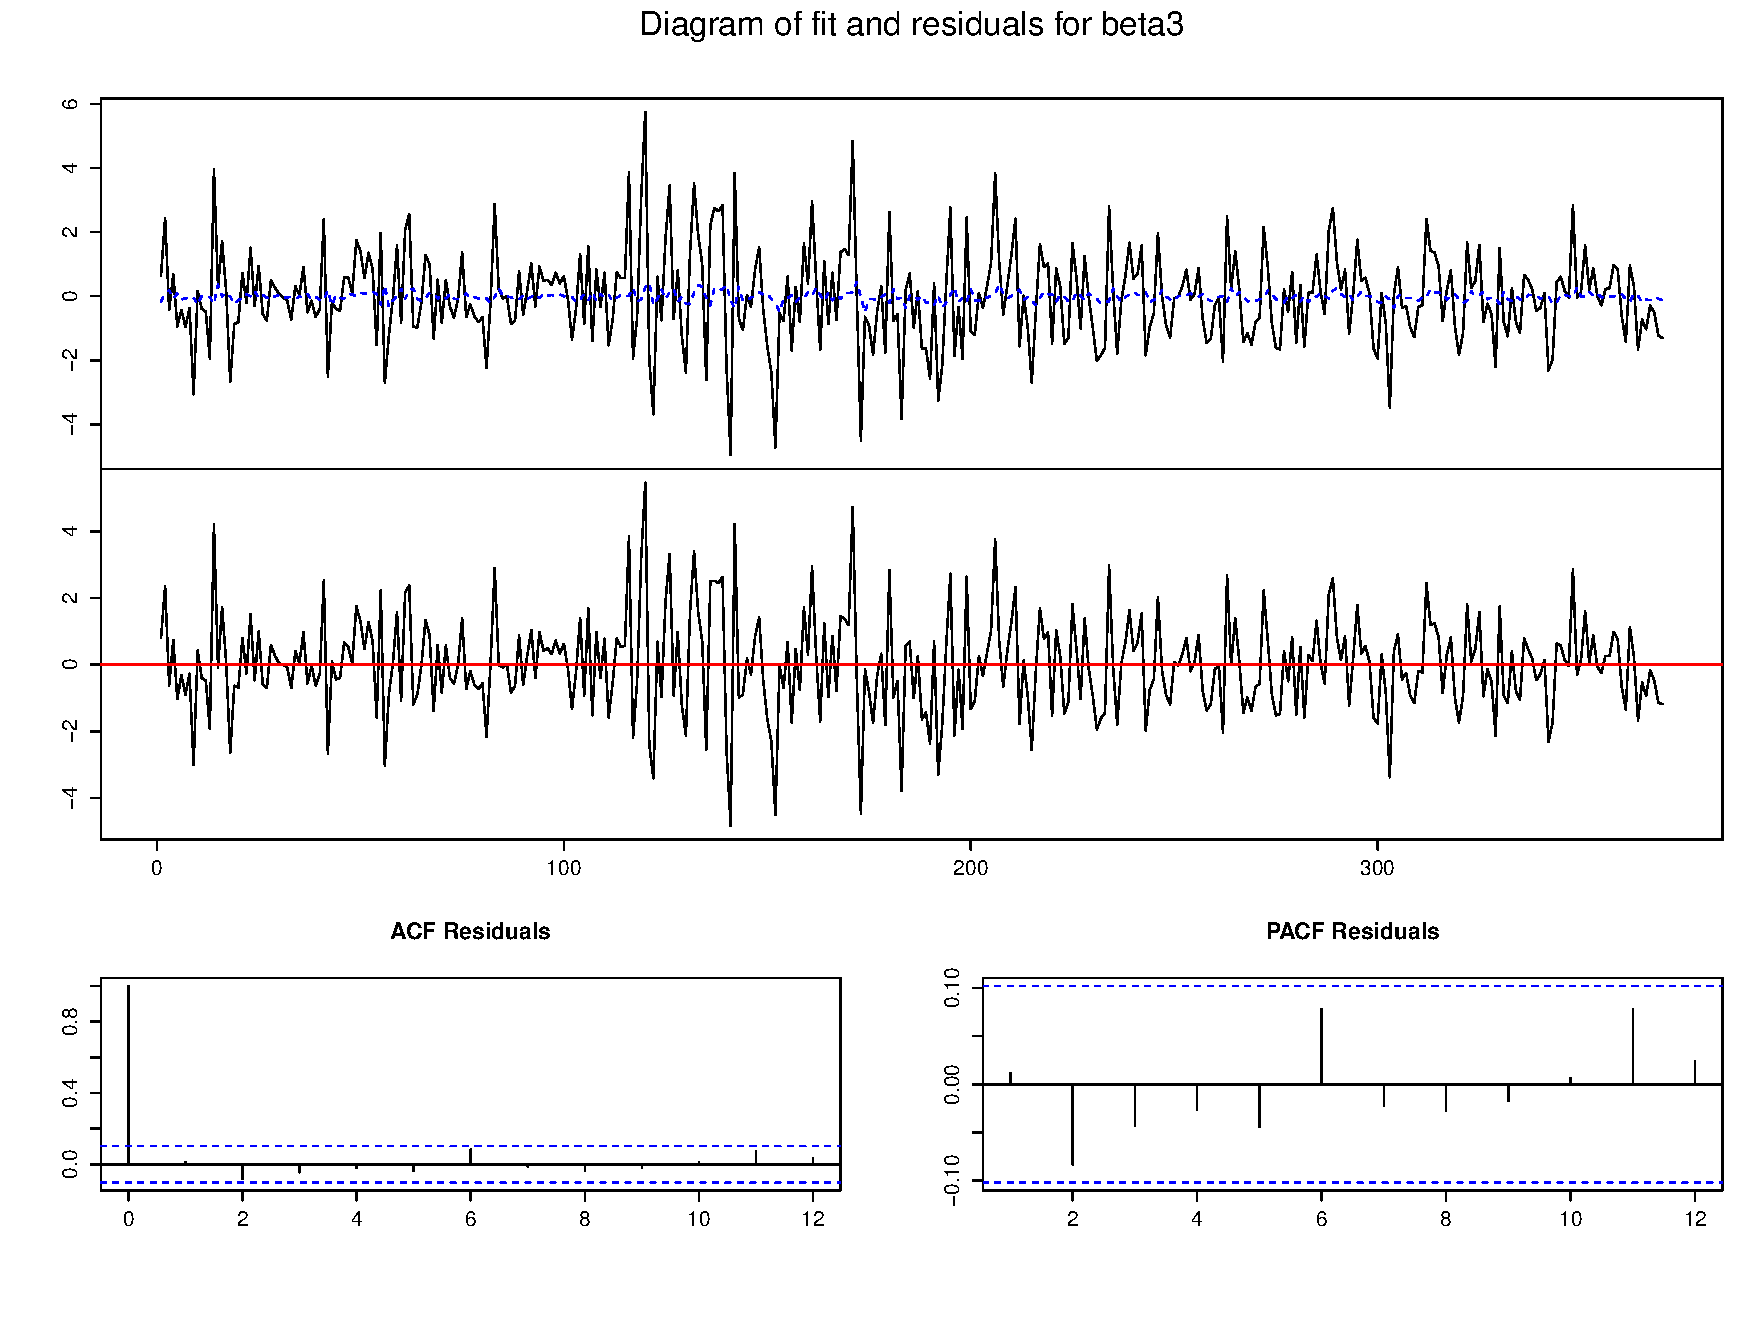
\includegraphics[width=15cm,height=15cm]{figures/Rplot14}
   \caption{一阶差分的曲度因子,$\Delta\hat{\beta}_{3t}$}
   \label{Rplot14}
  \end{figure}
 %------------------------------------------------------
 \subsubsection{残差分析}
 最后,\figref{Rplot15}和\figref{Rplot16}给出了残差图,表明残差符合白噪声随机过程(White Noise),即序列无关、服从高斯正态分布。
  %------------------------------------------------------
        \begin{figure}%[!h]
     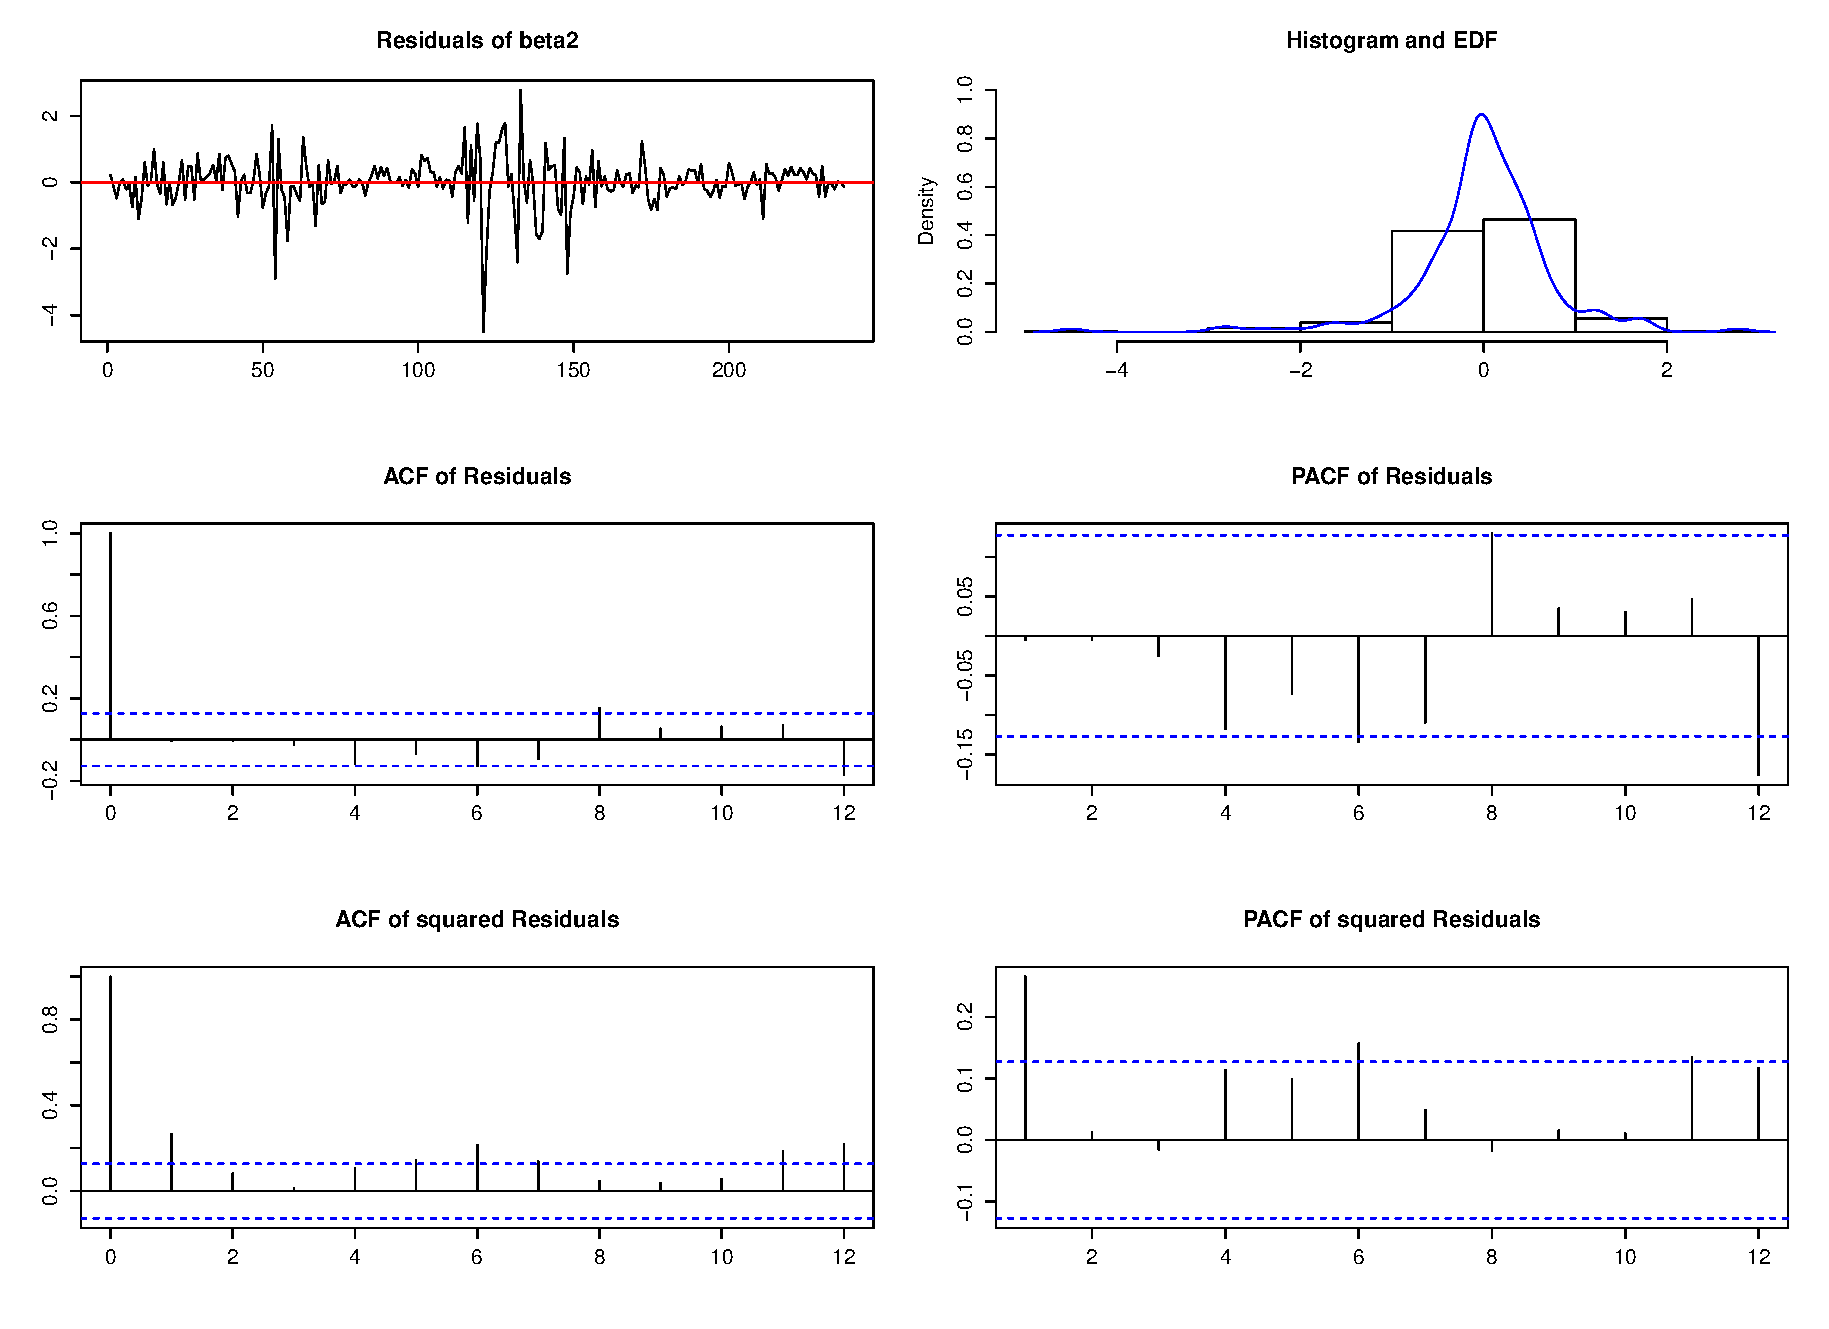
\includegraphics[width=15cm,height=15cm]{figures/Rplot15}
    \caption{$\Delta\hat{\beta}_{2t}$的残差项}
    \label{Rplot15}
   \end{figure}
   
    %------------------------------------------------------
          \begin{figure}%[!h]
       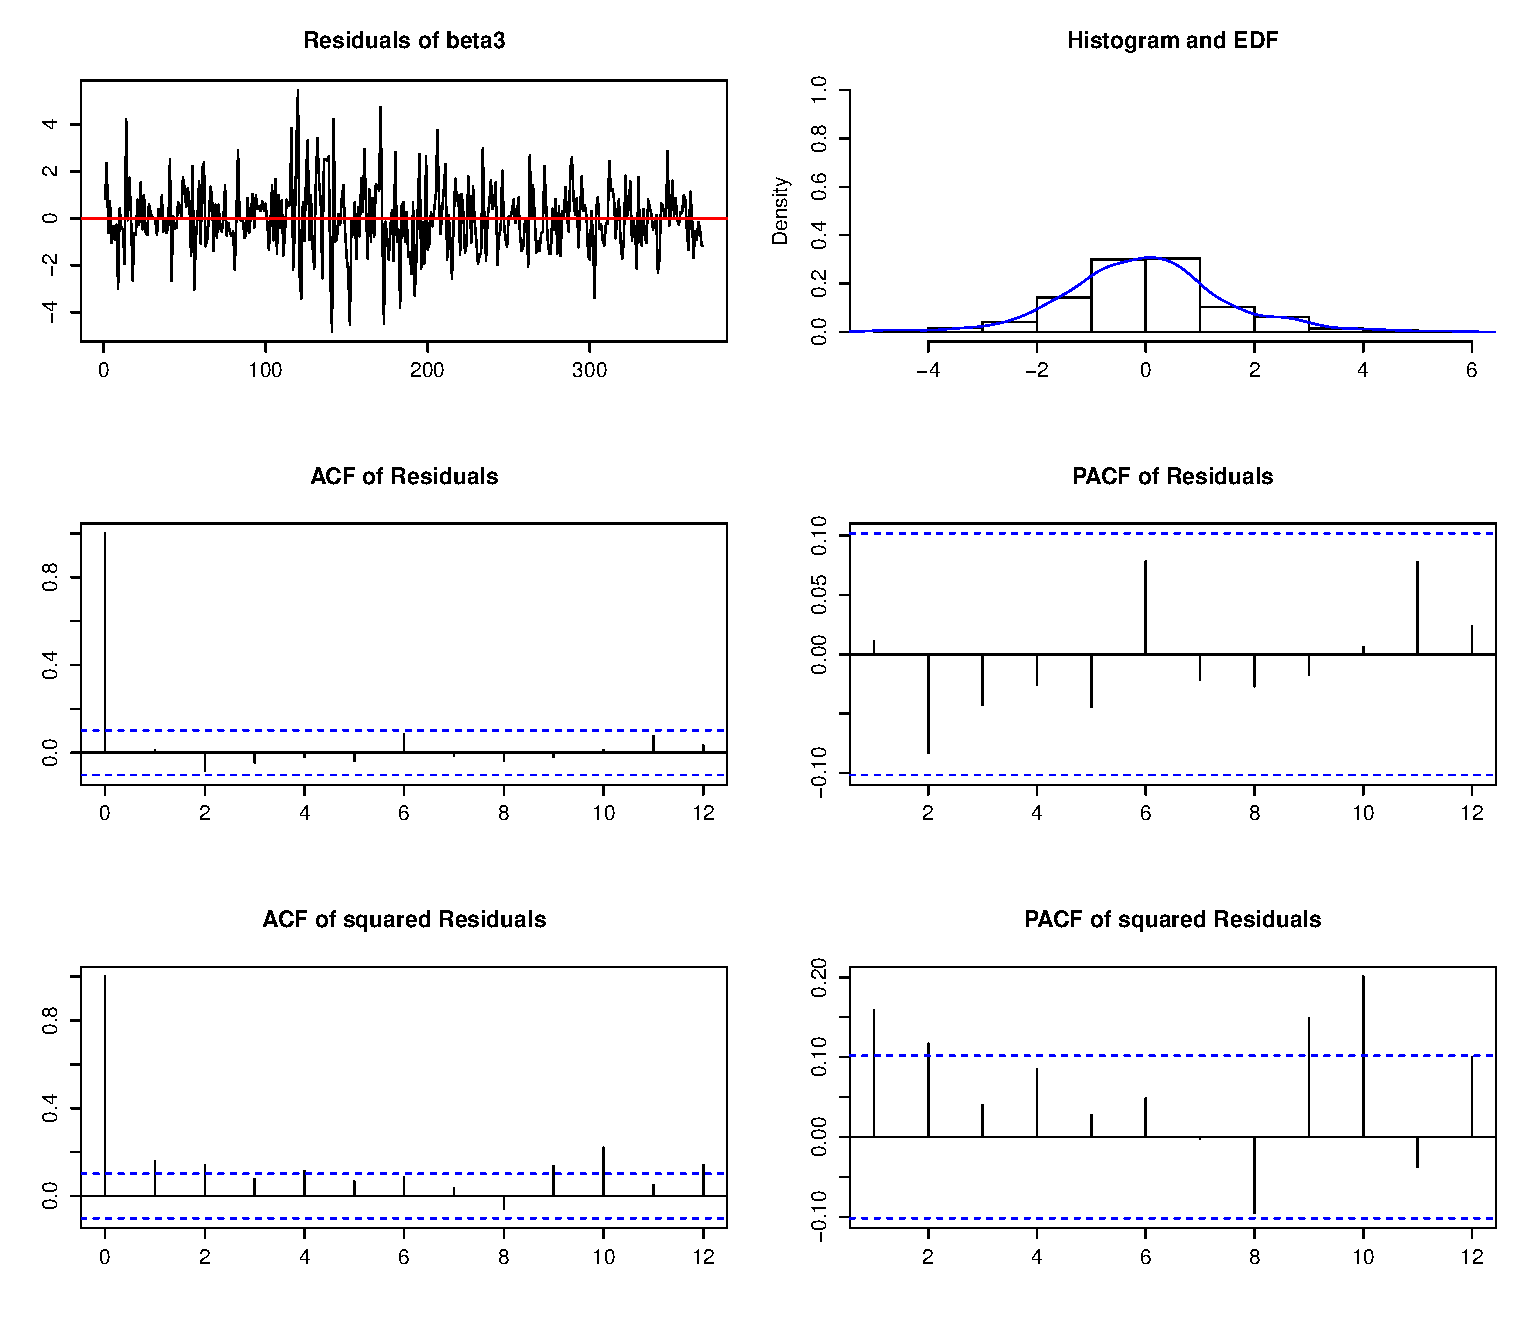
\includegraphics[width=15cm,height=15cm]{figures/Rplot16}
      \caption{$\Delta\hat{\beta}_{3t}$的残差项}
      \label{Rplot16}
     \end{figure}
 %------------------------------------------------------

\subsection{人口因子载荷分析}{Demographic Loading}
通过以上的第一步最小二乘回归,我们从而可以进一步分析人口趋势对利率期限结构的因子载荷。对于不同的到期日,我们分别估计出其相应的因子载荷,这些代表来人口因素对收益率曲线长期、稳定的影响。这可以用来解释收益率曲线中不能被短期与中期的斜率因子与曲度因子所解释的长期、平稳的部分变化。下文将进一步解释在利率期限结构模型中引入反映人口年龄结构变化的变量能够很好的捕捉到长期均衡利率的持久性组成部分,从而比传统的利率期限期限结构模型能更好地解释长期利率的变化。

 \begin{lstlisting}[language=R]
  yld.tilde <- yld - Beta %*% t(M)
  w <-matrix(, nrow = n.maturity, ncol = 1)  ## demographic loadings
  for ( i in 1:n.maturity ){
    w[i] <- coef(lm(yld.tilde[,i] ~ my[,i] - 1))
  }
  yld.fit <- matrix(, nrow = n.data, ncol = n.maturity)
  for (j in 1:n.data){
    for (i in 1:n.maturity){
      yld.fit[j,i] <- w[i] * my[j,i] + M[i,1] * Beta[j,1] + M[i,2] * Beta[j,2]
    }}
 \end{lstlisting}

\figref{Rplot10}给出来收益率曲线的因子载荷图形。我们知道,在\dns{}中,原来的三个影响收益率动态特征的因子分别为水平因子、斜率因子与曲度因子,即$\{\beta_{1t},\beta_{2t},\beta_{3t}\}$。但是,在本文之前,现有的文献几乎都将水平因子载荷设定为一个单位参数,即在长期不会对收益率曲线产生任何影响。显然,这个假定过于随意,缺乏说服力度。产生该问题的主要原因,还是在于现有的利率期限结构理论没有充分考虑到人口因素的结构性、宏观性、整体性的影响。
\begin{figure}\centering%[!h]
    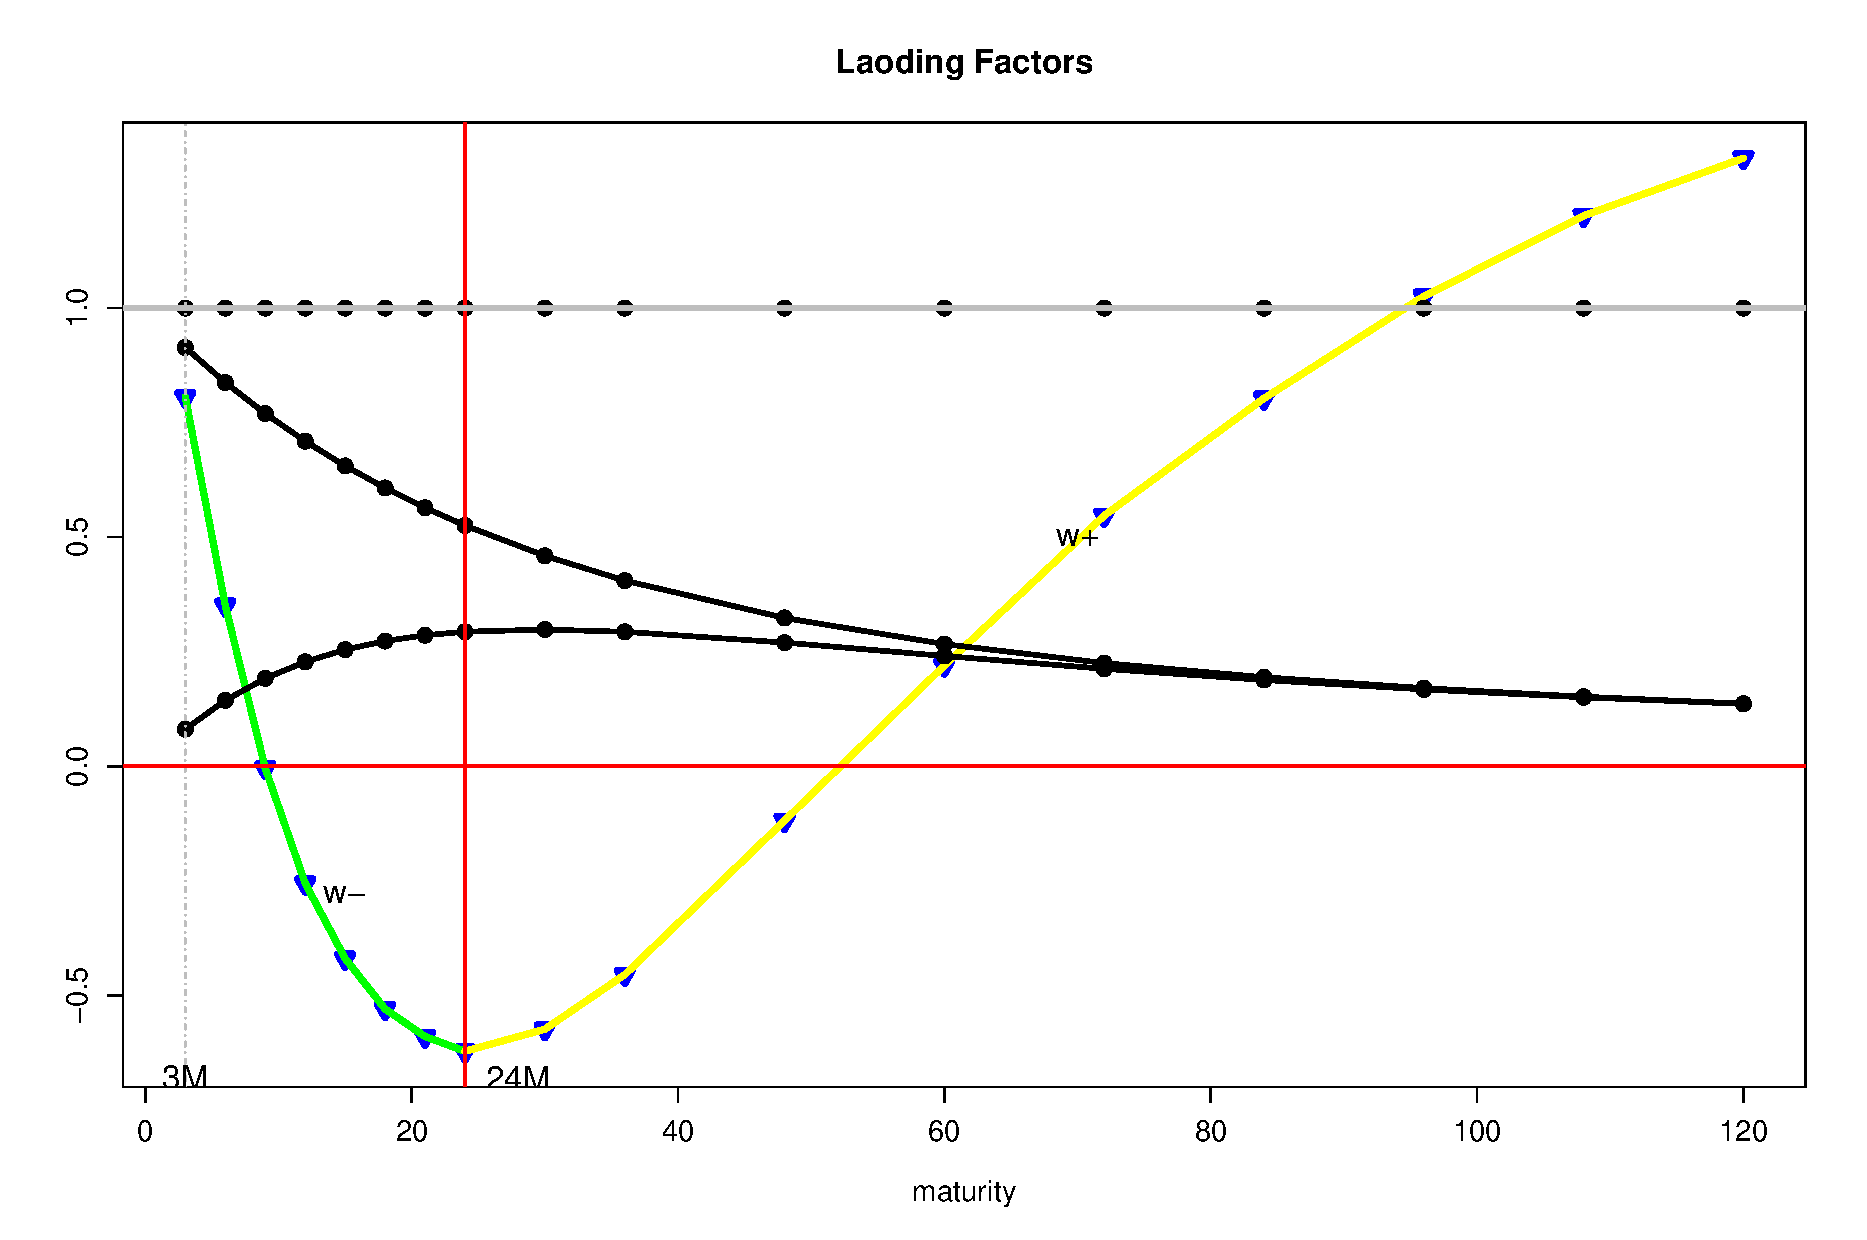
\includegraphics[width=15cm,height=9cm]{figures/Rplot10}
   \caption{人口因子载荷}
   \label{Rplot10}
  \end{figure}
  
在\figref{Rplot10}中,我们注意到人口因子载荷先是在短期内由正逐渐下降至负值(緑色线条),然后在逆向增加,并且在更长的到期日上升。
\begin{compactitem}
 \item 由于人口因素在短期内的变化不是很大,由其带来的对收益率曲线的影响相对较弱。用一个社会人群当中的中年人口与年轻人口的比率作为影响收益率曲线长期变化行为的因子,对于解释短期内的变动比较有限。我们知道,变量$MY_t$的变化是一个缓慢持久的过程,需要在大约为一个世代频率范畴内对经济产生久期的影响。而这个能够很好的解释一个家庭共同作为投资人在分散与规避风险方面的决策行为。这是目前金融研究中消费-资本资产定价理论(C-CAPM)。
 \item 通常,家庭为了对冲未来不确定带来的收入波动,需要将部份资产投资在风险相对较小、流动性较强的金融产品上。由政府、市政部门、企业公司等发行的债券类金融证券在短期内具有一定的波动性,但从长期来看,则具有相对风险小、流动性强等特征,而债券市场正是满足来家庭投资的需要。因此,从长期来看,经济社会当中的人口年龄变化趋势诱导着家庭金融理财行为,继而对债券的长期收益率曲线带来持久稳定的影响。
 \item 因此,将人口年龄结构变化引入到利率期限结构模型中,不仅有利于我们理解长期收益率曲线的动态变化特征,而且我们可以利用这种稳定而可预测的人口趋势来实现对未来收益率的预测。
\end{compactitem}

\section{收益率曲线拟合}{Yiled Curve Fitting}
使用带人口年龄结构变量的\dns 对实际的收益率进行拟合:
 \begin{align}
   \hat{y}_{t}(\tau) & = \hat{\omega}_t MY_{t}(\tau)
        + \hat{\beta}_{2t} \big[\frac{1-e^{-\lambda \tau}} {\lambda \tau} \big]
        + \hat{\beta}_{3t}\big[\frac{1-e^{-\lambda \tau}} {\lambda \tau} - e^{-\lambda \tau} \big].
 \end{align}
 这里,设定~$\lambda_t$~为~$0.0609$~从而使中期的曲度因子的载荷系数最大化\citep{diebold2006forecasting}。

\subsection{样本内拟合}{In-sample Fitting}

 \figref{Rplot02}刻画了人口年龄结构变量的\dns 对实际的收益率的样本内拟合情况。该图显示,在动态~Nelson-Siegel~模型中引入人口年龄结构变量,能够很好地对收益率曲线进行拟合。同样的,\figref{Rplot03}显示该模型能够对不同类型的收益率曲线做较好的样本拟合,如上升的收益率曲线、下降的收益率曲线以及呈拱形的收益率曲线。然而,注意到\figref{Rplot03}右下角显示的是~1989~年~5~月~31~日的国债收益率曲线,当日不同收益率呈现不规则的分布,因此,对其做的样本拟合并不是十分理想。这说明利用人口因素驱动的利率期限结构模型对于能够反映经济系统规律性的、长期的变化趋势比较敏感,而对于一些短暂的经济冲击则无法及时反馈。

%%
\begin{figure}\centering%[!h]
    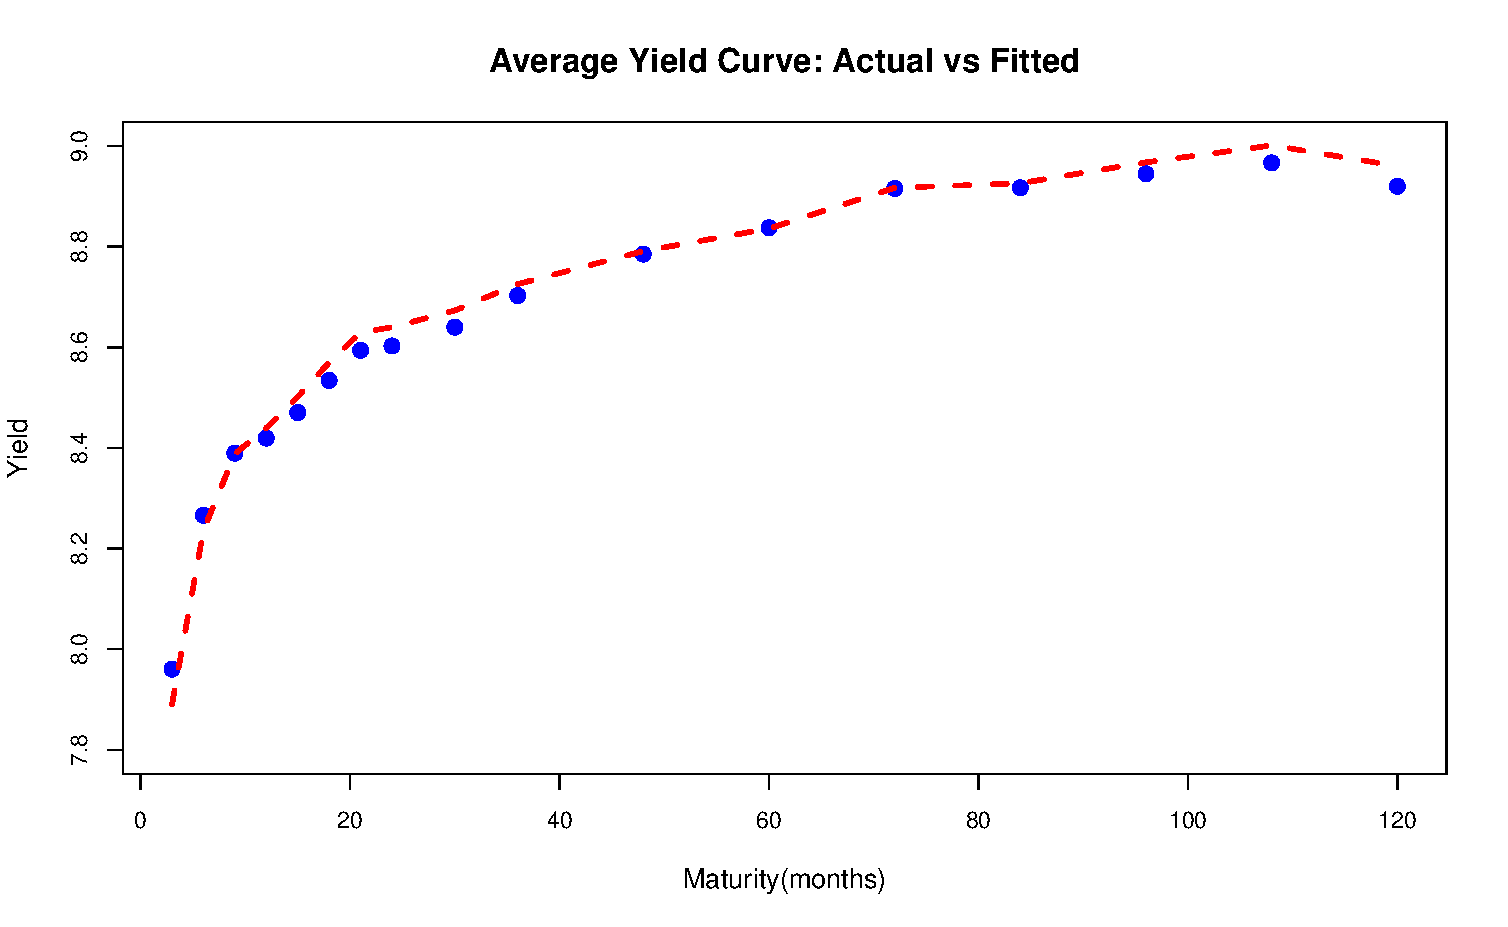
\includegraphics[width=15cm,height=9cm]{figures/Rplot02}
   \caption{收益率曲线的样本拟合情况:1970:01 - 1984:12。}
   \label{Rplot02}
  \end{figure}
       %%%%%%%%%%%%%%%%%%%%%%%%%%
  \begin{figure}%[!h]
      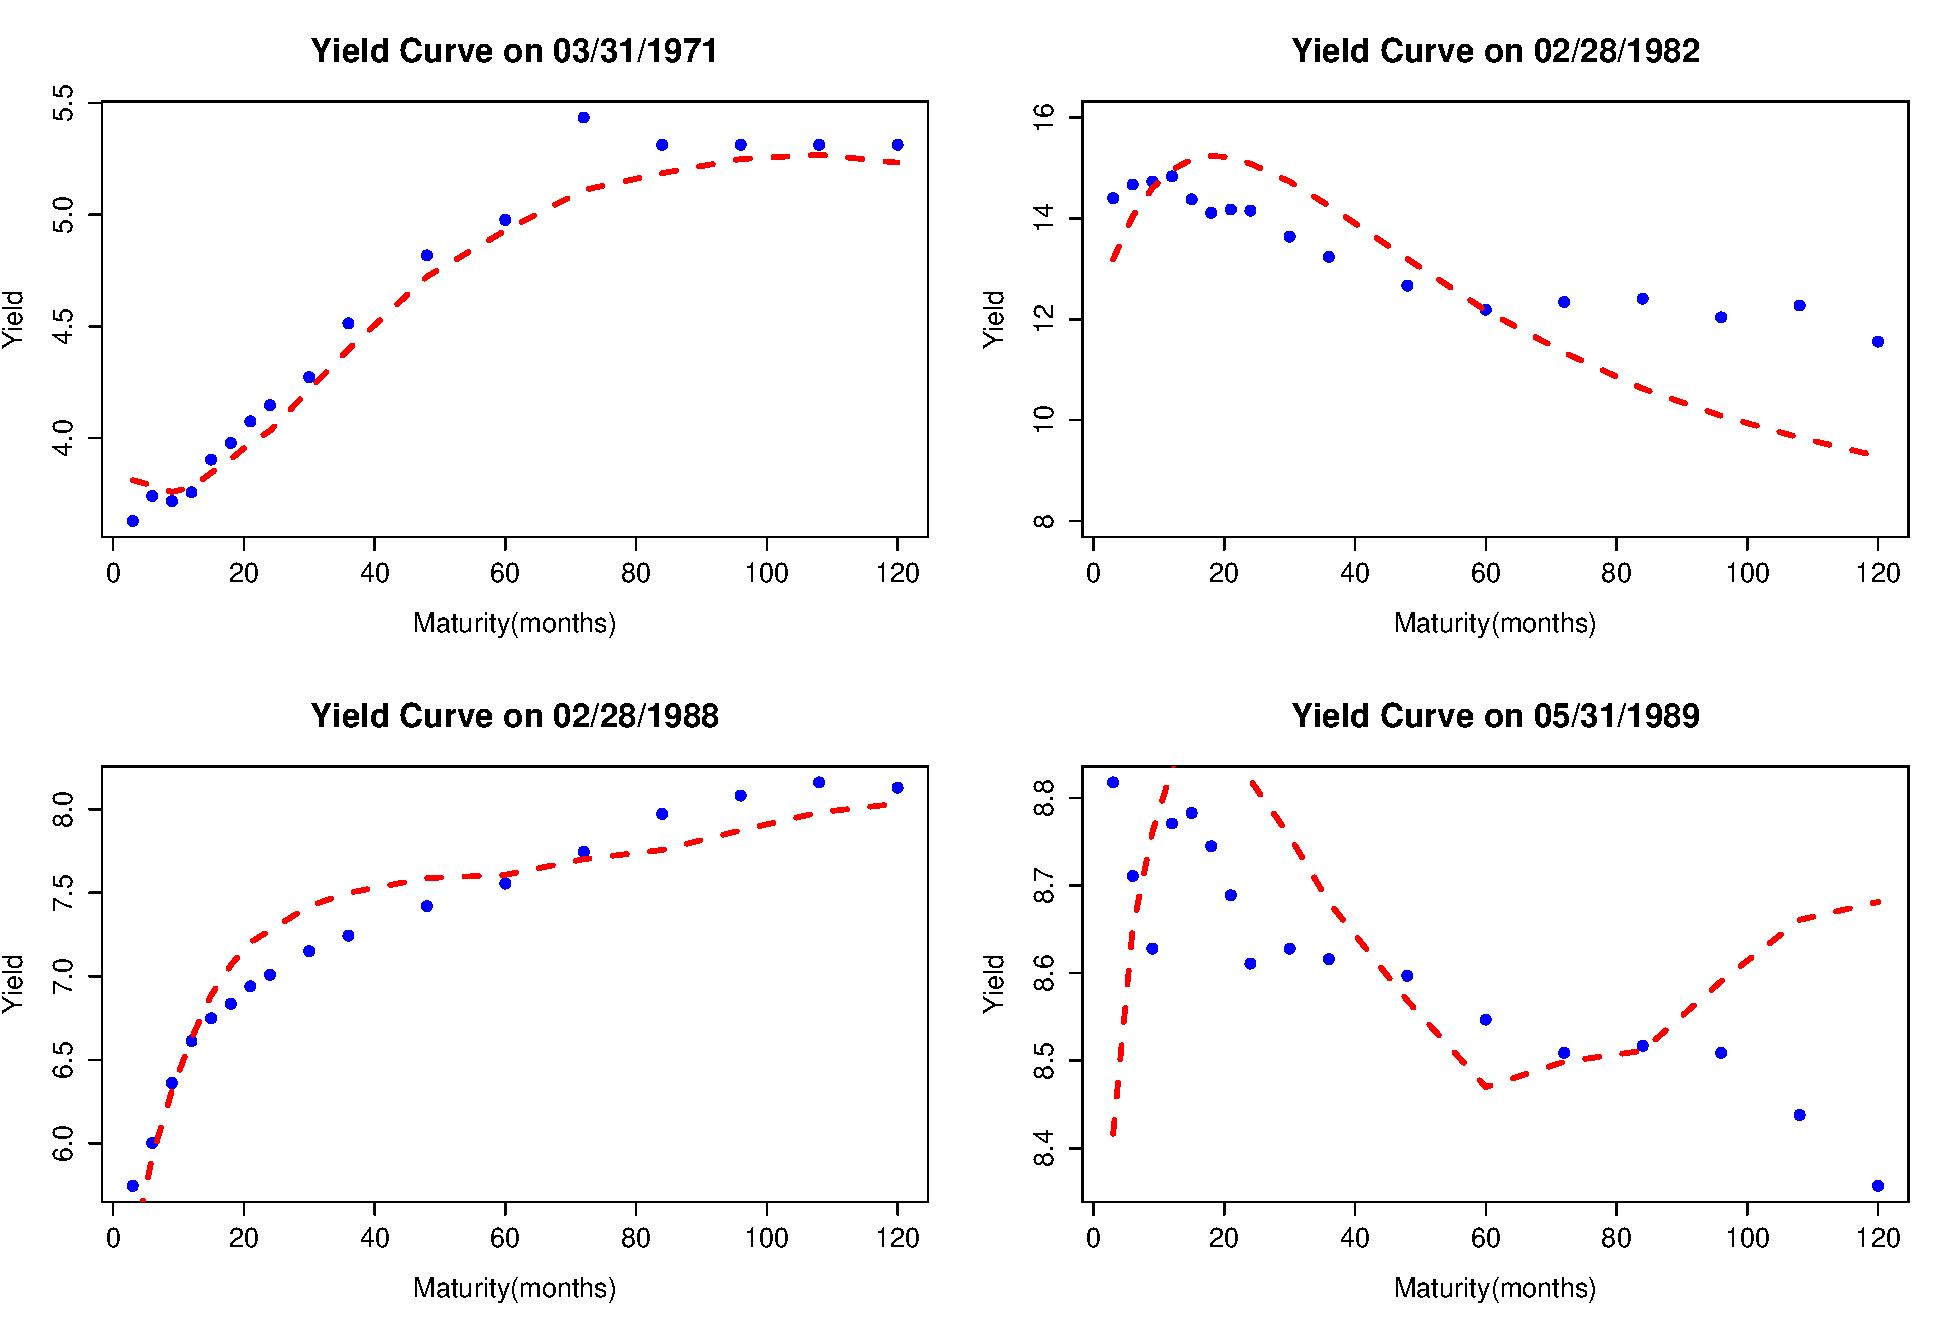
\includegraphics[width=15cm,height=12cm]{figures/Rplot03}
     \caption{特定时点上的收益率曲线拟合效果}
     \label{Rplot03}
    \end{figure} 
   %%
   
 \figref{Rplot04}对代表\tsm 的水平因子、斜度因子及曲度因子与模型估计的三个因子~$\{\hat{K}_{t}, \hat{\beta}_{2t}, \hat{\beta}_{3t}\}$~分别进行了拟合。在上图中,有人口年龄结构所决定的长期利率的平稳部分,$\hat{K}_{t}$,能够很好的捕捉到收益率曲线的水平变动情况,亦即货币市场对未来利率的理性预期。这点在\tabref{coefficients}中也得到了印证,估计得到的~$\hat{K}_{t}$~与实际收益率曲线的水平值的相关系数达到了~$0.9789$。这肯定了将人口年龄结构变量引入\tsm 能够很好地反映代表长期均衡利率的水平变动。而且,由于人口年龄结构的可预测性,这能够为预测未来利率提供很好的基础。
   %%
  \begin{figure}%[!h]
      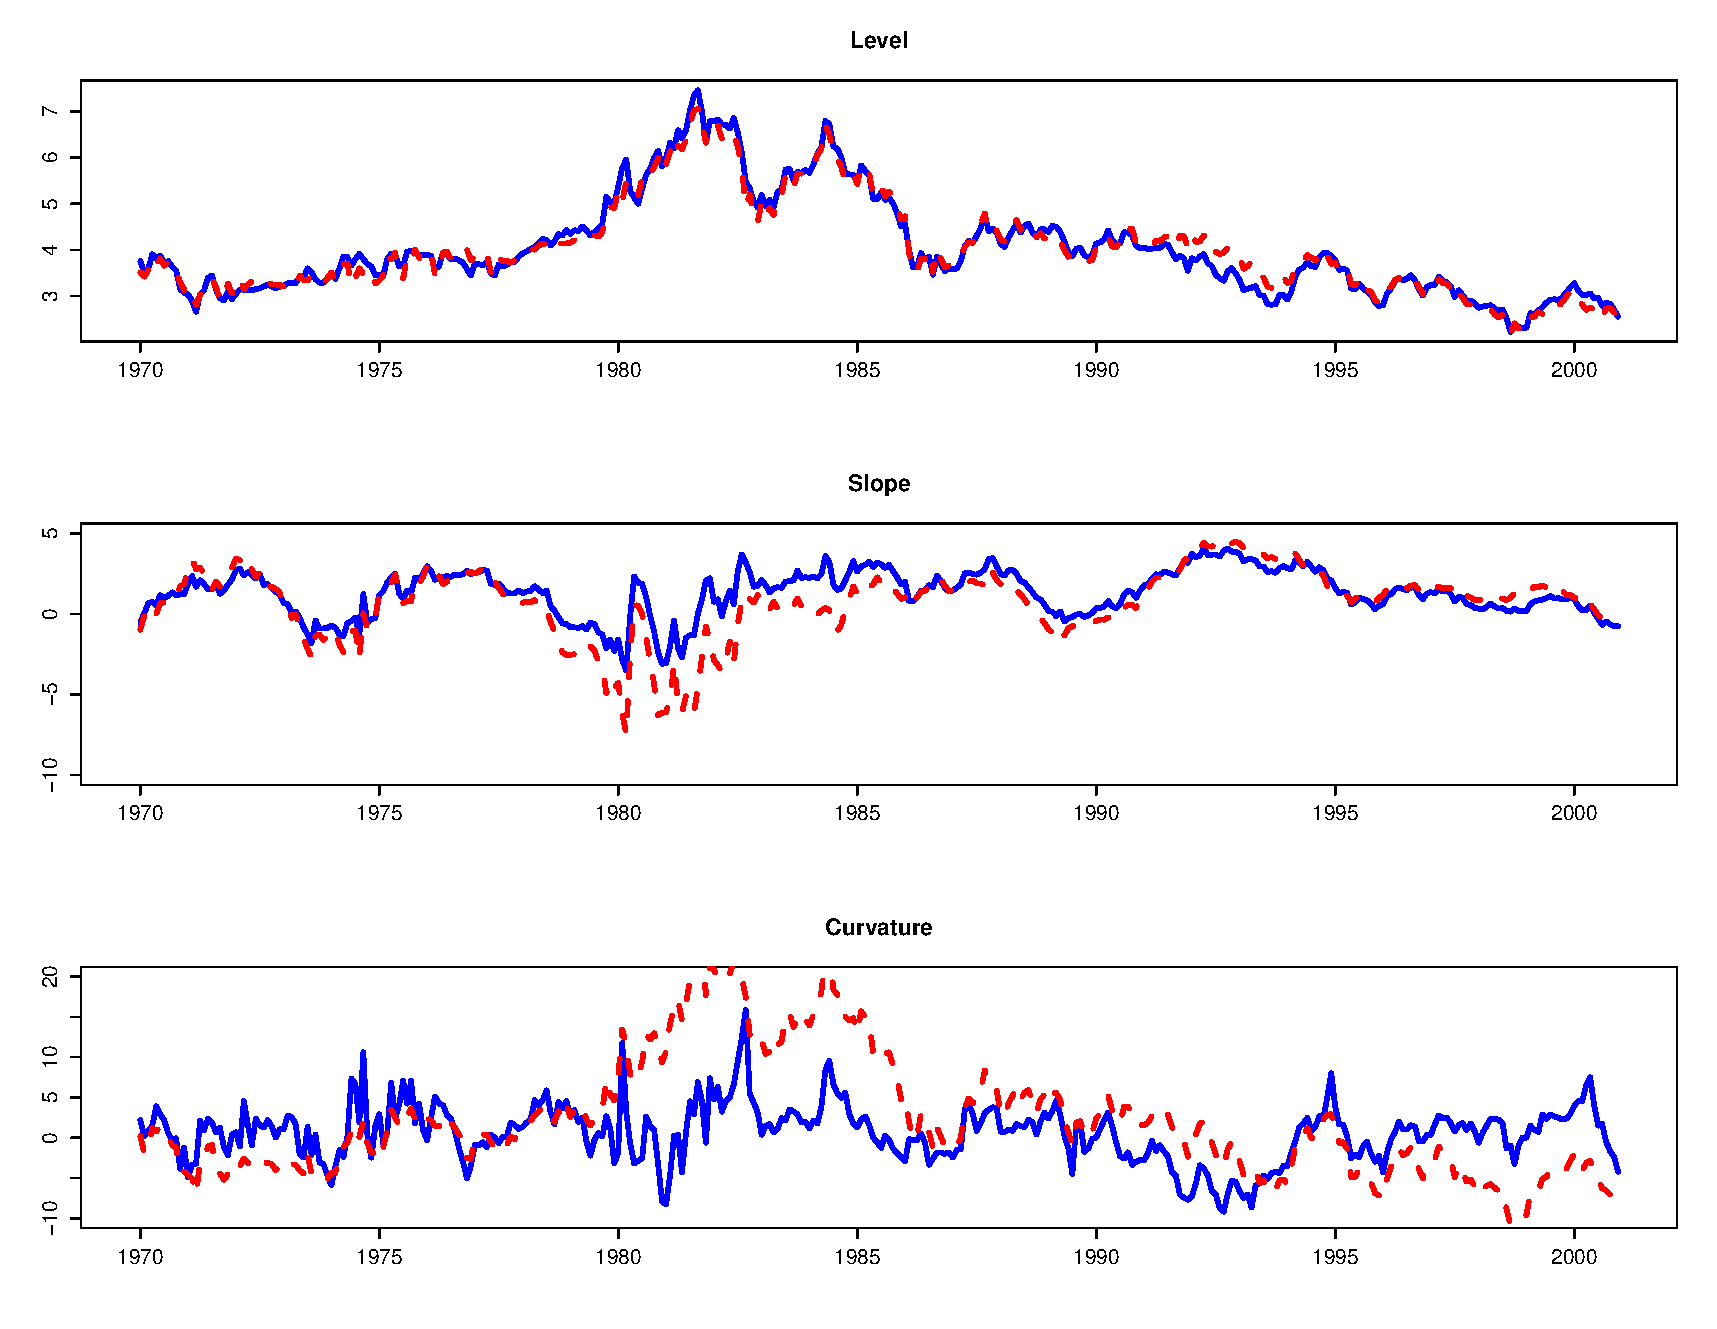
\includegraphics[width=15cm,height=22cm]{figures/Rplot04}
     \caption{短期、中期以及长期收益率拟合}
     \label{Rplot04}
 \end{figure}
 
 \subsection{收益率长期动态特征与人口因素}{Long-term Characteristics and Demographic Factors}
 
 为了更清楚的看出这个由人口年龄结构决定的平稳部分为何能够反映长期利率水平,\figref{Rplot06}给出在不同预测长度的~$\{\hat{K}_{t}(\tau)\}$~的预测值。随着到期期限增加,$\{\hat{K}_{t}(\tau)\}$~对收益亏曲线中的水平值的拟合越来越好。\figref{Rplot07}分别给出来不同期限长短的收益率曲线的拟合情况。可以看到,在短期内,由人口因素驱动的收益率曲线并不能很好的拟合实际收益率曲线,这些短期特征主要是受到斜率因子和曲度因子,$\{\beta_{2t},\beta_{3t}\}$影响;然而,由这两个因子所不能够捕捉的代表收益率曲线长期水平却能在由人口因素的模型下得到很好的解释,即在\figref{Rplot07}的第三部份,我们看到人口因素在一个较长的频率上良好的拟合来长期利率水平。
  
   \begin{figure}%[!h]
      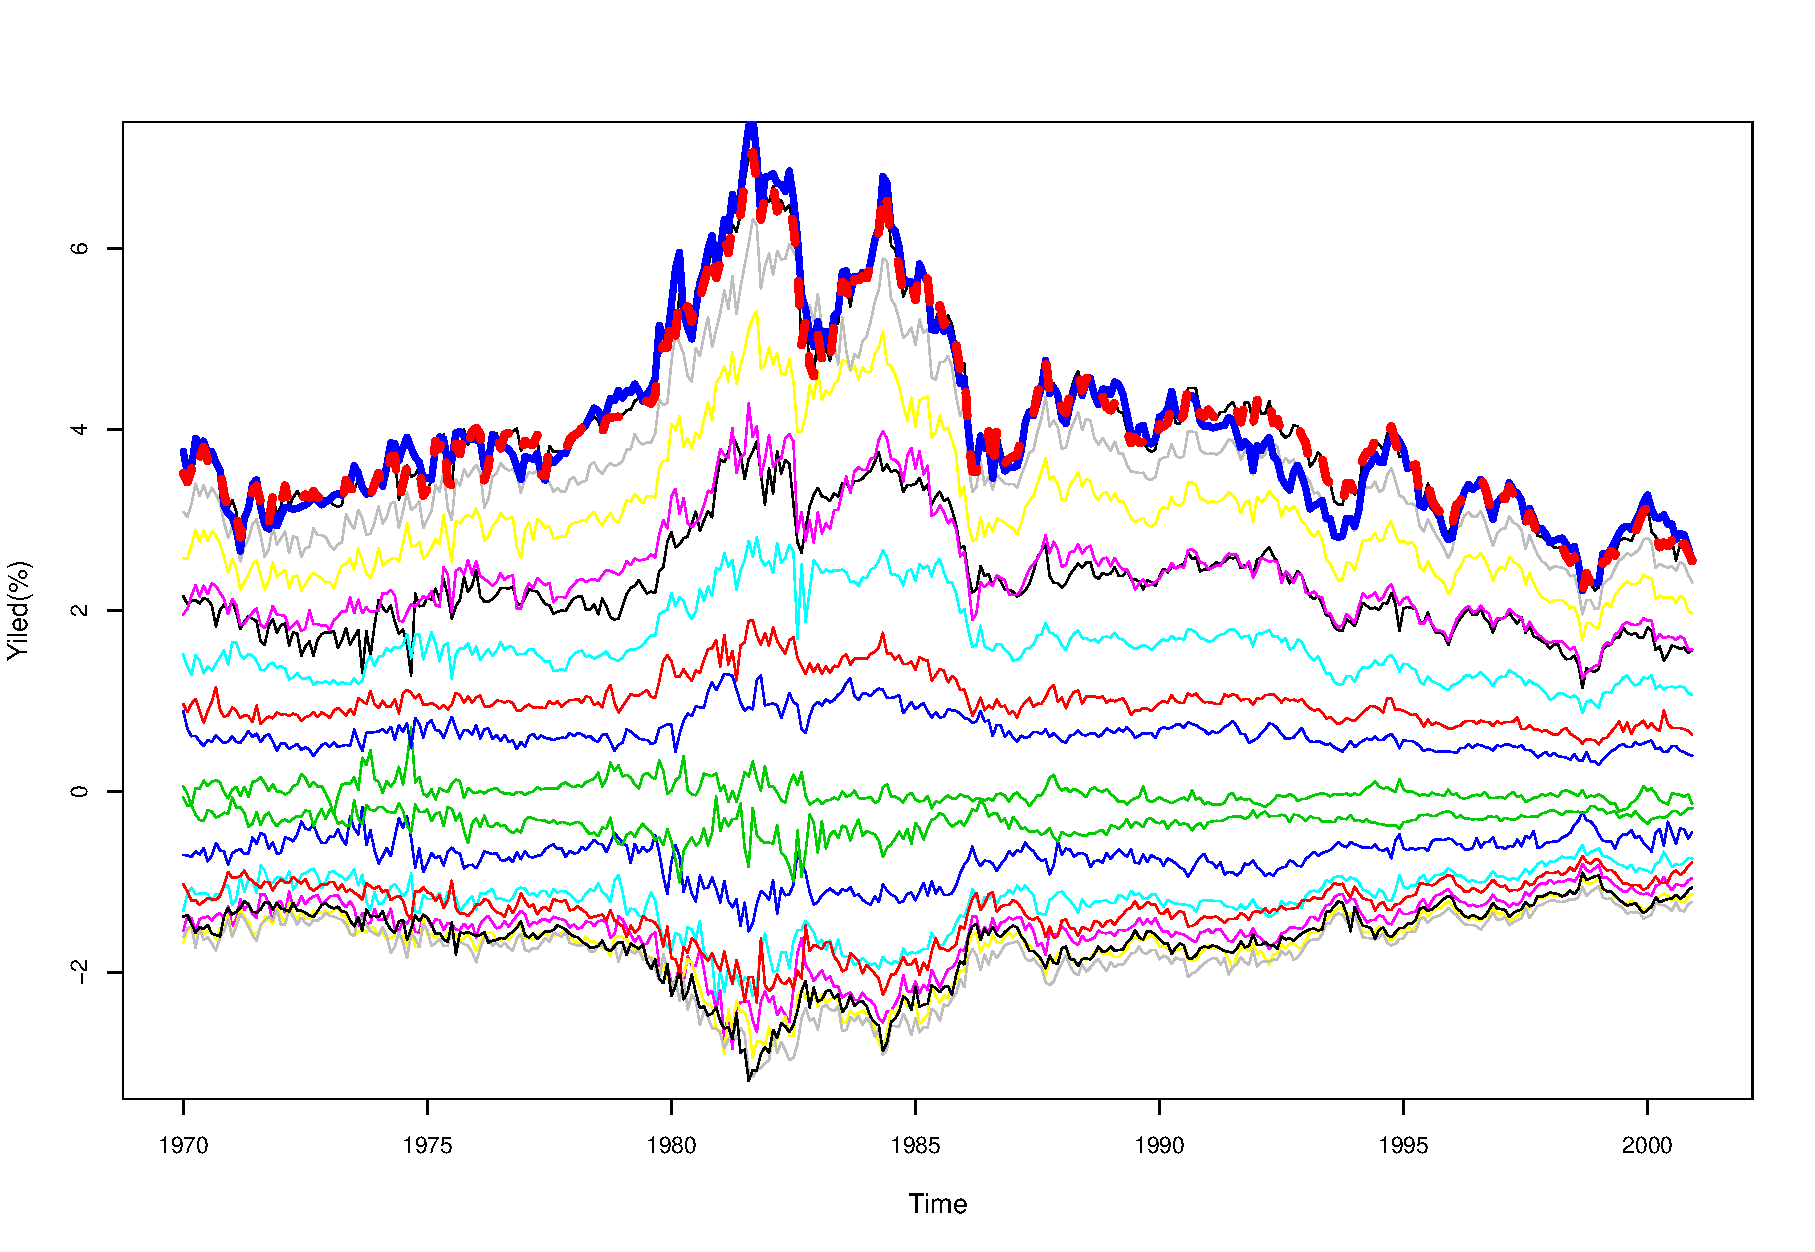
\includegraphics[width=15cm,height=8cm]{figures/Rplot06}
     \caption{利率中预测的久性平稳部分与利率水平值}
     \label{Rplot06}
    \end{figure} 
   %%
  \begin{figure}%[!h]
      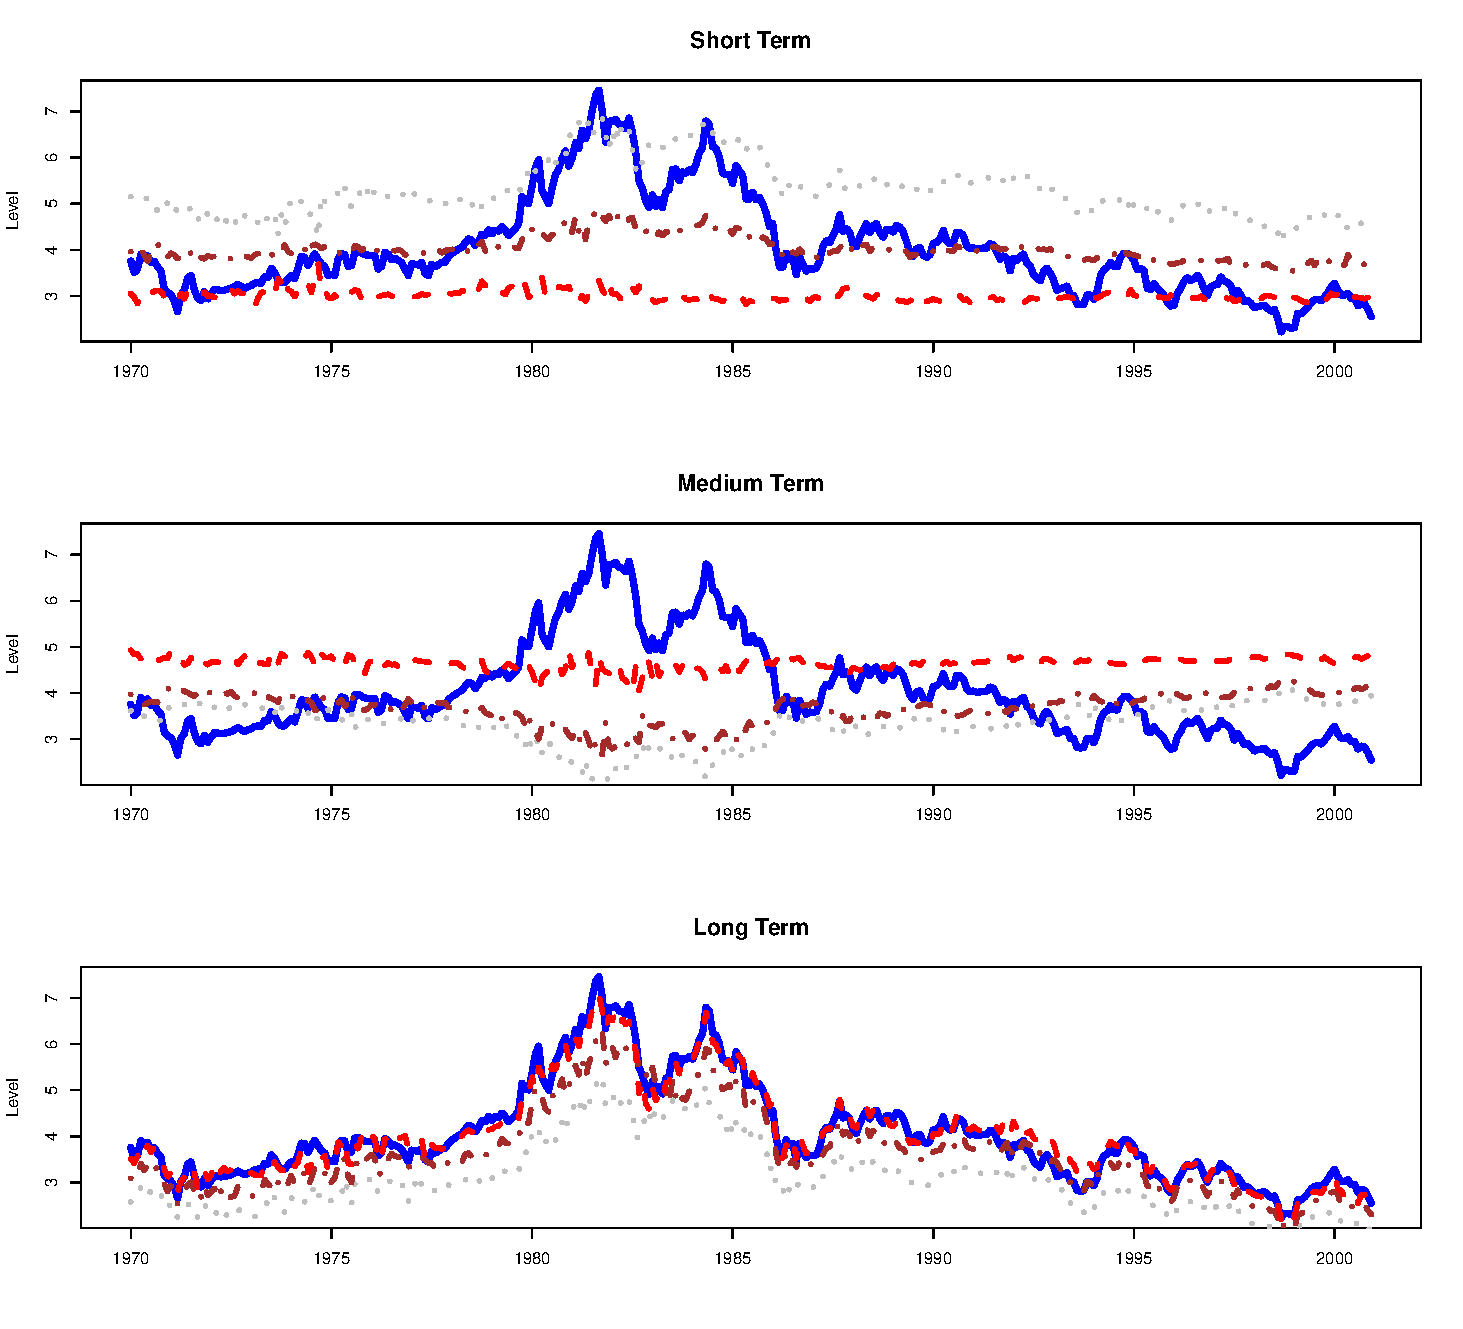
\includegraphics[width=15cm,height=20cm]{figures/Rplot07}
     \caption{收益率的平稳部分与不同到期日收益}
     \label{Rplot07}
 \end{figure}
   
 此外,\tabref{coefficients}显示~$\{\hat{K}_{t}(\tau)\}$~的自相关系数较高,滞后一期的自相关系数为~$0.979$,滞后~12~期的自相关系数仍然高达~$0.770$,这说明其在收益率曲线中确实能够反映出具有久性特征的长期利率水平的变动情况。
 
 对于另外两个影响因子,$\hat{\beta}_{2t}$~和~$\hat{\beta}_{3t}$,则代表了收益率的短期及中期行为。二者的自相关系数在短期内比较高,而随着和滞后期的增加,其自相关系数急剧下降,这也说明了两个影响因子只能刻画出收益率曲线在中短期的随机性行为特征,而无法反映利率在长期的动态特征。

 通过对模型参数的估计,可以得到一条对实际收益率较好拟合的曲线函数。这个由人口年龄结构驱动、并考虑了短期利率行为特征的\dns{}能够在样本内对实际收益率做很好的拟合分析,并给估计得到的参数也可以给以合理的经济学解释。因此,下一章将利用此模型来对未来收益率曲线做样本外的预测。

  %%
 \begin{center}
  \begin{threeparttable}\vspace{-.6cm}
  %%
 \caption{估计的影响因子与实际因子的相关关系}
 \label{coefficients}
 \renewcommand{\arraystretch}{1.2} \arrayrulewidth=0.8pt \tabcolsep=6pt
\begin{tabular}{@{}ccccccccccc@{}} 
\hline \hline 
  & $\hat{K}_t$ & $\hat{\beta}_{2t}$  & $\hat{\beta}_{3t}$
        & $L$  & $S$  & $C$  & $\hat{\rho}(1)$ & $\hat{\rho}(3)$ & $\hat{\rho}(12)$ & $\hat{\rho}(30)$ \\ \hline
$\hat{K}_t$ & $1$ &  &  & &  &   &   0.979     &    0.945     &    0.770     &   0.539      \\ 
$\hat{\beta}_{2t}$ & $$-$0.459$ & $1$ &   &   &   &  & 0.955 & 0.852 & 0.579  & 0.049 \\ 
$\hat{\beta}_{3t}$ & $$-$0.964$ & $0.459$ & $1$ &   &   &   & 0.976 & 0.927 & 0.760 & 0.540\\ 
L & $0.984$ & $$-$0.567$ & $$-$0.984$ & $1$ &   &  &        &         &         &          \\ 
S & $0.046$ & $0.858$ & $$-$0.042$ & $$-$0.076$ & $1$ &   &        &         &         &         \\ 
C & $0.206$ & $$-$0.265$ & $$-$0.429$ & $0.333$ & $$-$0.083$ & $1$ &        &         &         &         \\ 
\hline \hline
\end{tabular} 
 %%
  \small{%
  \emph{注}: 在R中自相关系数的统计置信区间为~$95\%$。
  }
\end{threeparttable}\end{center}




